\documentclass[11pt,a4paper]{article}

\usepackage{lmodern}
\usepackage[T1,T5]{fontenc}
\usepackage[utf8]{inputenc}
\usepackage[margin=0.92in]{geometry}
\usepackage{amsmath,amssymb,amsfonts}
\usepackage{booktabs,multirow,tabularx,array}
\usepackage{graphicx}
\usepackage{float}
\usepackage{xcolor}
\usepackage[numbers,sort&compress]{natbib}
\usepackage[unicode]{hyperref}

\definecolor{navy}{RGB}{20,45,90}
\definecolor{crimson}{RGB}{165,30,45}
\definecolor{teal}{RGB}{0,110,110}

\hypersetup{
    colorlinks=true,
    linkcolor=navy,
    citecolor=teal,
    urlcolor=crimson,
    pdftitle={Hoc may Tich hop Ly thuyet Kinh te (EIML) trong Du bao Kiet que Tai chinh Doanh nghiep},
    pdfauthor={Nhom Nghien cuu Rui ro Tin dung Dinh luong}
}

\renewcommand{\figurename}{Hình}
\renewcommand{\tablename}{Bảng}
\renewcommand{\refname}{Tài liệu tham khảo}
\renewcommand{\abstractname}{Tóm tắt (Abstract)}

\setlength{\parskip}{0.38em}
\setlength{\parindent}{1.2em}

\title{\vspace{-1.2cm}\textbf{\Large Học máy Tích hợp Lý thuyết Kinh tế trong Dự báo Kiệt quệ Tài chính Doanh nghiệp: Ràng buộc Cấu trúc Nhúng và Bằng chứng Thực nghiệm Ngoài mẫu Thời gian tại Việt Nam}\\[0.35em]
\large\textit{(Economically-Informed Machine Learning for Corporate Financial Distress Prediction: Embeddable Structural Constraints and Out-of-Time Evidence from Vietnam)}}

\author{
    \textbf{Nhóm Nghiên cứu Rủi ro Tín dụng Định lượng \& Học máy Tài chính}\\
    \small\textit{Thiết kế theo Quy trình Đa tác tử Google Research PaperOrchestra chuẩn Q1}\\
    \small\textit{Tạp chí mục tiêu: Expert Systems with Applications / International Review of Financial Analysis}
}
\date{Tháng 11 năm 2026}

\begin{document}
\maketitle

\begin{abstract}
\noindent
Dự báo kiệt quệ tài chính doanh nghiệp (Corporate Financial Distress Prediction) là một trụ cột cốt lõi của tài chính doanh nghiệp thực nghiệm và quản trị rủi ro tín dụng. Mặc dù các bộ phân loại học máy (Machine Learning -- ML) dung lượng cao --- như cây quyết định tăng cường độ dốc (GBDT) và mạng nơ-ron đa tầng sâu (MLP) --- thường xuyên vượt trội hơn các mô hình chấm điểm tuyến tính cổ điển trên dữ liệu bảng kế toán, chúng lại mắc phải hai lỗ hổng cấu trúc nghiêm trọng cản trở việc áp dụng trong giám sát an toàn vĩ mô tại các thị trường mới nổi. Thứ nhất, các bộ ước lượng phi tuyến không ràng buộc thường khớp quá mức vào các tương quan giả tạo, phi đơn điệu trong các tỷ số kế toán nhiễu, dẫn đến các kết quả tĩnh học so sánh trái ngược với lý thuyết kinh tế (ví dụ: dự báo xác suất vỡ nợ giảm xuống khi tỷ lệ đòn bẩy nợ tăng lên) và vi phạm các biên thanh toán cấu trúc. Thứ hai, các nghiên cứu thực nghiệm về kiệt quệ tài chính thường mắc phải \textit{thiên kiến nhìn trước} (look-ahead bias) nghiêm trọng xuất phát từ việc kiểm định chéo $K$-fold ngẫu nhiên cắt ngang qua các năm dữ liệu bảng, cắt cụt ngoại lai (winsorization) và nội suy trên toàn bộ mẫu, trộn lẫn dữ liệu lịch sử hồi tố trước khi niêm yết (pre-IPO backfilling), và thiên kiến sống sót (survivorship bias) khi các doanh nghiệp vỡ nợ bị hủy niêm yết. Để giải quyết đồng thời cả hai thách thức này, chúng tôi đề xuất khung \textbf{Học máy Tích hợp Lý thuyết Kinh tế (Economically-Informed Machine Learning -- EIML)} gồm hai nhánh bổ trợ: (i) mô hình cây \textbf{Monotonic GBDT} với ràng buộc dấu đạo hàm tại từng nút phân tách, và (ii) \textbf{Mạng Nơ-ron Tích hợp Lý thuyết Kinh tế khả vi (Proposed EINN)} áp đặt tính đơn điệu từng phần thông qua tái tham số hóa trọng số bằng hàm softplus kết hợp với hàm phạt biên cấu trúc lấy cảm hứng từ lý thuyết định giá nợ của Merton và vùng mất khả năng thanh toán của Altman. Được kiểm định trên bộ dữ liệu bảng 15 năm đã qua kiểm toán pháp y gồm $11.455$ quan sát doanh nghiệp--năm ($7.602$ cặp chuyển trạng thái hậu niêm yết của $692$ doanh nghiệp phi tài chính trên HOSE, HNX và UPCOM giai đoạn 2008--2022) theo giao thức chia tách ngoài mẫu thời gian tuyệt đối (strict out-of-time) bao phủ cuộc khủng hoảng trái phiếu doanh nghiệp và hủy niêm yết năm 2021--2022 tại Việt Nam ($N_{\text{test}}=2.083$), khung EIML đạt hiệu năng phân loại hàng đầu đồng thời triệt tiêu hoàn toàn các vi phạm tiên đề kinh tế. Trong bài toán dự báo chuyển trạng thái kiệt quệ mới trước 1 năm (Chế độ A: $Y_{i,t+1}^{\text{fwd}}$), \textbf{Monotonic GBDT} đạt $\text{ROC-AUC} = 0,8021$, $\text{PR-AUC} = 0,3793$, điểm Brier $= 0,0798$ và Điểm Nhất quán Kinh tế ($\text{ECS}$) đạt $99,97\%$; trong khi \textbf{Proposed EINN} cải thiện $\text{PR-AUC}$ thêm $+4,96\%$ so với mạng MLP không ràng buộc ($0,3517$ so với $0,3021$) và nâng điểm $\text{ECS}$ từ $29,00\%$ lên $100,00\%$ ($0,00\%$ vi phạm đơn điệu và biên). Trong bài toán dự báo kiệt quệ đa kỳ dai dẳng (Chế độ B: $Y_{i,t+1}^{\text{ovl}}$), \textbf{Monotonic GBDT} và \textbf{Proposed EINN} đạt $\text{ROC-AUC}$ lần lượt là $0,9648$ và $0,9592$ với độ nhất quán kinh tế $100,00\%$, cảnh báo sớm thành công các tổ chức phát hành rơi vào khủng hoảng năm 2022 (\texttt{FLC}, \texttt{HAI}, \texttt{BII}, \texttt{AMD}, \texttt{GAB} và \texttt{VKC}) từ báo cáo tài chính năm 2021.

\vspace{0.5em}
\noindent\textbf{Từ khóa:} Dự báo kiệt quệ tài chính doanh nghiệp; Học máy tích hợp lý thuyết kinh tế (EIML); Mạng nơ-ron đơn điệu; Rủi ro tín dụng cấu trúc; Thiên kiến nhìn trước (Look-Ahead Bias); Doanh nghiệp niêm yết Việt Nam.
\vspace{0.3em}\\
\noindent\textbf{Phân loại JEL:} C45, C52, C53, G17, G32, G33.
\end{abstract}

% =========================================================================
% PHẦN 1: GIỚI THIỆU (INTRODUCTION)
% =========================================================================
\section{Giới thiệu (Introduction)}
\label{sec:intro}

Dự báo chính xác, kịp thời và có thể giải thích được về mặt kinh tế đối với tình trạng kiệt quệ tài chính doanh nghiệp có ý nghĩa sống còn đối với các ngân hàng thương mại, trái chủ, cơ quan giám sát an toàn vĩ mô và nhà đầu tư cổ phiếu \citep{beaver1966financial,altman1968financial,campbell2008search}. Tại các thị trường vốn mới nổi, nơi cơ chế thực thi công bố thông tin đang trong quá trình hoàn thiện, độ bao phủ xếp hạng tín nhiệm độc lập còn hạn chế và cấu trúc nợ doanh nghiệp phụ thuộc nặng nề vào tín dụng ngân hàng ngắn hạn cùng trái phiếu doanh nghiệp phát hành riêng lẻ, các làn sóng mất khả năng thanh toán đột ngột có thể kích hoạt sự đóng băng thanh khoản mang tính hệ thống \citep{altman1995emerging,pham2018financial,tran2023examining}. Tính dễ tổn thương này đã bộc lộ rõ nét trong cuộc khủng hoảng thanh khoản trái phiếu doanh nghiệp và bất động sản tại Việt Nam giai đoạn 2021--2022, khi việc mở rộng đòn bẩy ngắn hạn quá mức kết hợp với khả năng chi trả lãi vay từ hoạt động cốt lõi suy yếu đã dẫn đến hàng loạt vụ vỡ nợ trái phiếu, đình chỉ giao dịch và hủy niêm yết bắt buộc trên Sở Giao dịch Chứng khoán TP.HCM (HOSE) và Sở Giao dịch Chứng khoán Hà Nội (HNX).

Về mặt lịch sử, tổng quan nghiên cứu dự báo vỡ nợ doanh nghiệp phát triển theo hai hệ hình phương pháp luận chính. Hệ hình thứ nhất bao gồm các mô hình thống kê cổ điển và mô hình rủi ro tín dụng cấu trúc, khởi đầu từ phân tích tỷ số đơn biến \citep{beaver1966financial}, phân tích biệt số đa biến ($Z$-score và $Z''$-score) \citep{altman1968financial,altman1995emerging,altman2017financial}, mô hình logit và probit có điều kiện \citep{ohlson1980financial,zmijewski1984methodological}, mô hình hàm nguy cơ rời rạc đa kỳ (discrete-time hazard models) \citep{shumway2001forecasting,chava2004bankruptcy,campbell2008search,bauer2014are}, và các mô hình khoảng cách đến vỡ nợ (distance-to-default) dựa trên lý thuyết định giá quyền chọn của \citet{merton1974pricing} \citep{hillegeist2004assessing,duffie2007multi,bharath2008forecasting}. Nhờ áp đặt dạng hàm tham số chặt chẽ và các tính chất tĩnh học so sánh rõ ràng, các mô hình này đáp ứng tốt yêu cầu kiểm toán của cơ quan quản lý; tuy nhiên, dạng hàm cộng tuyến tính của chúng không thể nắm bắt được các tương tác phi tuyến phức tạp giữa cấu trúc kỳ hạn nợ, sự suy giảm vốn lưu động và dòng tiền hoạt động.

Hệ hình thứ hai khai thác các bộ phân loại học máy (ML) phi tham số và học sâu (Deep Learning) --- bao gồm rừng ngẫu nhiên (Random Forest) \citep{breiman2001random}, cây quyết định tăng cường độ dốc (GBDT) \citep{chen2016xgboost,ke2017lightgbm,prokhorenkova2018catboost}, máy vectơ hỗ trợ (SVM) và mạng nơ-ron sâu \citep{lessmann2015benchmarking,zieba2016ensemble,barboza2017machine,mai2019deep,hosaka2019bankruptcy,gunnarsson2021deep}. Mặc dù các mô hình tổ hợp ML dung lượng cao liên tục đạt độ chính xác xếp hạng vượt trội trên các bộ dữ liệu chuẩn, chúng lại tạo ra một mâu thuẫn căn bản giữa tính linh hoạt dự báo và tính hợp lý kinh tế \citep{bussmann2021explainable,bucker2022transparency,dumitrescu2022machine}. Khi được huấn luyện trên dữ liệu bảng kế toán nhiễu và có đuôi dày tại các thị trường mới nổi, các mô hình ML không ràng buộc thường xuyên vi phạm các tiên đề nền tảng của tài chính doanh nghiệp. Cụ thể, một mạng MLP không ràng buộc hoặc RBF-SVM có thể khớp các dao động cục bộ khiến cho việc gia tăng tỷ lệ nợ trên tổng tài sản ($\text{Debt}/\text{Assets}$) hoặc tỷ trọng nợ ngắn hạn ($\text{ShortDebt}/\text{TotalDebt}$) trong điều kiện các yếu tố khác không đổi (ceteris paribus) lại làm \textit{giảm} xác suất vỡ nợ dự báo. Hơn nữa, tại các vùng biên ngoài phân phối (out-of-distribution tails), các bộ phân loại không ràng buộc thường gán xác suất kiệt quệ cao cho các doanh nghiệp gần như không có nợ và có lãi (vi phạm biên an toàn nợ bằng không của Merton) hoặc gán xác suất rủi ro thấp cho các doanh nghiệp đã âm vốn chủ sở hữu.

Làm trầm trọng thêm thách thức mô hình hóa này là một lỗ hổng phương pháp luận phổ biến trong các nghiên cứu ML tài chính thực nghiệm: \textit{thiên kiến nhìn trước} (look-ahead bias / rò rỉ thông tin) và quy trình làm sạch dữ liệu bảng thiếu chặt chẽ \citep{bailey2014pseudo,lopez2018advances}. Qua kiểm toán pháp y đối với các nghiên cứu dự báo kiệt quệ tài chính tại thị trường mới nổi và Việt Nam gần đây \citep[ví dụ:][]{pham2018financial,vo2019corporate,tran2022explainable,tran2023examining,vu2023lasso}, chúng tôi xác định bốn nguồn rò rỉ và sai lệch nghiêm trọng:
\begin{enumerate}
    \item \textbf{Chia tách ngẫu nhiên cắt ngang và lấy mẫu quá mức (SMOTE) trên toàn mẫu theo thời gian:} Việc áp dụng kiểm định chéo $K$-fold ngẫu nhiên hoặc chia ngẫu nhiên $70/30$ (thường kết hợp với SMOTE trên toàn bộ mẫu) cắt ngang qua dữ liệu bảng nhiều năm cho phép các quan sát ở năm $t+k$ tham gia huấn luyện để dự báo cho năm $t$, làm rò rỉ các cú sốc vĩ mô tương lai và trạng thái kiệt quệ dai dẳng của cùng một doanh nghiệp vào tập huấn luyện.
    \item \textbf{Độ trễ công bố báo cáo và rò rỉ từ công thức tỷ số đồng nhất thức (tautology):} Theo quy định công bố thông tin trên thị trường chứng khoán Việt Nam, báo cáo tài chính năm đã kiểm toán của năm tài chính $t$ được công bố trong vòng 90 ngày sau khi kết thúc năm (tức đến ngày 31/03 của năm $t+1$). Ngoài ra, khi chi phí lãi vay bị khuyết, việc nội suy ngây thơ hoặc tính $\text{EBIT} = \text{NetProfit} + |\text{InterestExpense}|$ sẽ biến điều kiện $\text{ICR} < 1,0 \iff \text{NetProfit} < 0$ thành một đồng nhất thức đại số (tautology) $100\%$.
    \item \textbf{Nhiễu từ dữ liệu hồi tố trước khi niêm yết (Pre-IPO backfilling):} Các cơ sở dữ liệu tài chính thương mại thường hồi tố 3--5 năm báo cáo tài chính trước thời điểm doanh nghiệp chính thức niêm yết ($\text{Year} < \text{Listedyear}$). Việc gộp các quan sát tiền IPO vào tập mẫu rủi ro tín dụng niêm yết làm sai lệch tỷ lệ vỡ nợ cơ sở.
    \item \textbf{Thiên kiến sống sót do hủy niêm yết bắt buộc (Survivorship bias):} Các doanh nghiệp rơi vào kiệt quệ nghiêm trọng ở năm $t$ và sau đó bị hủy niêm yết hoặc không nộp báo cáo tài chính ở năm $t+1$ thường bị các đoạn mã ghép trễ (lag-alignment) loại bỏ vô tình, làm mất đi các ca vỡ nợ tín dụng nghiêm trọng nhất.
\end{enumerate}

Lấy cảm hứng từ các tiến bộ mới nhất về học máy tích hợp vật lý (Physics-Informed Machine Learning -- PINNs) \citep{raissi2019physics,karniadakis2021physics} và mạng nơ-ron đơn điệu \citep{sill1997monotonic,you2017deep,runje2023constrained}, bài báo này bắc cầu nối giữa học máy dung lượng cao và lý thuyết rủi ro tín dụng cấu trúc. Chúng tôi phát triển khung \textbf{Học máy Tích hợp Lý thuyết Kinh tế (EIML)} và kiểm định trên bộ dữ liệu bảng 15 năm đã qua làm sạch pháp y của các doanh nghiệp phi tài chính niêm yết tại Việt Nam (2008--2022). Bốn đóng góp cốt lõi của bài báo bao gồm:
\begin{itemize}
    \item \textbf{Kiến trúc Học máy Tích hợp Kinh tế Hai nhánh (Dual-Track EIML):} Chúng tôi thiết lập hệ hình EIML nhúng trực tiếp các tiên đề rủi ro tín dụng cấu trúc vào cả mô hình tổ hợp cây (\textbf{Monotonic GBDT}) và mạng nơ-ron sâu (\textbf{Proposed EINN}). Bằng cách kết hợp tái tham số hóa trọng số softplus trên các tập biến đơn điệu ($\mathcal{M}_+, \mathcal{M}_-$) với hàm mục tiêu phức hợp phạt các vi phạm tại biên an toàn nợ bằng không của Merton và biên mất khả năng thanh toán của Altman, Proposed EINN đảm bảo $0,00\%$ vi phạm đơn điệu và $0,00\%$ vi phạm biên ($\text{ECS} = 100,00\%$).
    \item \textbf{Quy trình Làm sạch Pháp y 7 bước và Tái cấu trúc Lợi nhuận Hoạt động ($\text{EBIT}_{\text{op}}$):} Chúng tôi xây dựng quy trình kiểm toán dữ liệu 7 bước giải quyết cột trùng lặp, nối mã chứng khoán bị đứt gãy (\texttt{MCO} $\to$ \texttt{MCG}), chuẩn hóa dấu của 40 dòng chi phí bị đảo dấu dương, cô lập $1.570$ dòng dữ liệu tiền IPO, triệt tiêu đồng nhất thức $\text{ICR} \iff \text{NetProfit}$ thông qua $\text{EBIT}_{\text{op}}$, và thu giữ 19 ca vỡ nợ hủy niêm yết hậu IPO.
    \item \textbf{Phân tách Dự báo Chuyển trạng thái Kiệt quệ Mới và Kiệt quệ Dai dẳng:} Chúng tôi tách bạch rõ ràng bài toán dự báo chuyển trạng thái kiệt quệ mới trước 1 năm của các doanh nghiệp đang lành mạnh (Chế độ A: $Y_{i,t+1}^{\text{fwd}}$, nơi $\text{AUC}$ thực tế đạt $\approx 0,77\text{--}0,81$) với bài toán kiệt quệ đa kỳ dai dẳng (Chế độ B: $Y_{i,t+1}^{\text{ovl}}$, nơi $\text{AUC}$ đạt $\approx 0,95\text{--}0,96$), lý giải nguyên nhân vì sao các nghiên cứu trước đây trộn lẫn hai chế độ lại báo cáo mức $\text{AUC}$ cao giả tạo.
    \item \textbf{Giải thích Tiên đề (Axiomatic XAI) và Kiểm toán Cảnh báo sớm Khủng hoảng Trái phiếu 2022:} Sử dụng phương pháp Tích phân Độ dốc (Integrated Gradients) \citep{sundararajan2017axiomatic}, chúng tôi chứng minh rằng mạng MLP không ràng buộc mắc tỷ lệ đảo dấu đạo hàm tới $67,16\%$ trên biến $\text{Debt}/\text{Assets}$ và $31,11\%$ trên biến $\text{EBIT}_{\text{op}}/\text{Assets}$, trong khi Proposed EINN triệt tiêu hoàn toàn hiện tượng đảo dấu ($0,00\%$) và phát tín hiệu cảnh báo sớm chính xác cho các doanh nghiệp tâm điểm khủng hoảng năm 2022 (\texttt{FLC}, \texttt{HAI}, \texttt{BII}, \texttt{AMD}, \texttt{GAB} và \texttt{VKC}) chỉ từ báo cáo tài chính năm 2021.
\end{itemize}

Phần còn lại của bài báo được cấu trúc như sau: Mục~\ref{sec:literature} tổng hợp cơ sở lý thuyết và tổng quan tài liệu theo 4 cụm chủ đề. Mục~\ref{sec:data} trình bày quy trình làm sạch dữ liệu pháp y, tái cấu trúc tỷ số hoạt động và thiết lập chia tách thời gian chống nhìn trước. Mục~\ref{sec:methodology} mô hình hóa toán học khung EIML, các tiên đề cấu trúc và chỉ số ECS. Mục~\ref{sec:experiments} phân tích kết quả thực nghiệm ngoài mẫu, nghiên cứu cắt bỏ (ablation study), giải thích XAI và kiểm toán khủng hoảng năm 2022. Mục~\ref{sec:conclusion} kết luận và đề xuất hàm ý chính sách.

% =========================================================================
% PHẦN 2: TỔNG QUAN TÀI LIỆU & ĐỊNH VỊ LÝ THUYẾT
% =========================================================================
\section{Tổng quan Tài liệu và Định vị Lý thuyết (Related Work)}
\label{sec:literature}

Tuân thủ quy trình tổng hợp theo chủ đề của \texttt{HybridLiteratureAgent}, chúng tôi hệ thống hóa tài liệu học thuật thành bốn dòng nghiên cứu liên kết chặt chẽ: (1) các mô hình kế toán cổ điển, mô hình hazard động và rủi ro tín dụng cấu trúc; (2) học máy tổ hợp và học sâu trong dự báo kiệt quệ tài chính; (3) học máy đơn điệu, mạng nơ-ron tích hợp lý thuyết và AI giải thích được (XAI); và (4) thiên kiến nhìn trước, vệ sinh dữ liệu bảng cùng các nghiên cứu thực nghiệm tại Việt Nam. Bảng~\ref{tab:lit_positioning} định vị phương pháp luận của bài báo so với các công trình chuẩn Q1--Q4 tiêu biểu.

\subsection{Mô hình Tỷ số Kế toán Cổ điển, Mô hình Hazard và Rủi ro Tín dụng Cấu trúc}
Dòng nghiên cứu thực nghiệm về dự báo phá sản doanh nghiệp khởi nguồn từ \citet{beaver1966financial}, người chứng minh rằng tỷ số dòng tiền trên tổng nợ và lợi nhuận ròng trên tổng tài sản có khả năng phân loại đơn biến mạnh mẽ trước khi doanh nghiệp vỡ nợ. \citet{altman1968financial} mở rộng cách tiếp cận này sang phân tích biệt số đa biến (MDA) với mô hình $Z$-score 5 nhân tố, và sau đó hiệu chỉnh cho các doanh nghiệp phi sản xuất và thị trường mới nổi thông qua mô hình $Z''$-score 4 nhân tố (Emerging Market Score -- EMS) \citep{altman1995emerging,altman2017financial}. Nhằm khắc phục giả định phân phối chuẩn khắt khe của MDA và ước lượng trực tiếp xác suất vỡ nợ, \citet{ohlson1980financial} và \citet{zmijewski1984methodological} lần lượt giới thiệu mô hình logit có điều kiện ($O$-score) và probit có trọng số. \citet{shumway2001forecasting} chứng minh rằng các mô hình phá sản tĩnh một kỳ tạo ra ước lượng chệch và không vững do bỏ qua thời gian chịu rủi ro, từ đó đặt nền móng cho mô hình hàm nguy cơ rời rạc đa kỳ (discrete-time hazard model) được mở rộng với hiệu ứng ngành \citep{chava2004bankruptcy}, biến số vĩ mô \citep{tinoco2013financial,bauer2014are} và tín hiệu thị trường tần suất cao \citep{campbell2008search}.

Song song đó, dòng lý thuyết rủi ro tín dụng cấu trúc khởi xướng bởi \citet{merton1974pricing} và lý thuyết đánh đổi cấu trúc vốn \citep{kraus1973state,myers1984capital} mô hình hóa vốn chủ sở hữu như một quyền chọn mua kiểu châu Âu (European call option) trên tổng tài sản của doanh nghiệp với giá thực hiện bằng mệnh giá nợ. Trong khung lý thuyết của Merton và các mở rộng thực nghiệm \citep{hillegeist2004assessing,duffie2007multi,bharath2008forecasting}, vỡ nợ xảy ra khi giá trị tài sản giảm xuống dưới ngưỡng nợ tới hạn, hàm ý các tính chất tĩnh học so sánh nghiêm ngặt: xác suất vỡ nợ là hàm không giảm theo đòn bẩy nợ ($\partial P / \partial (D/A) \ge 0$) và là hàm không tăng theo khả năng sinh lời hoạt động cũng như độ bao phủ dòng tiền ($\partial P / \partial \text{ROA} \le 0$). Hơn nữa, do thủ tục phá sản pháp lý tại các thị trường mới nổi thường kéo dài nhiều năm, \citet{asquith1994anatomy}, \citet{pindado2008estimating} và \citet{tinoco2013financial} đã thiết lập chuẩn mực định nghĩa kiệt quệ tài chính dựa trên sự mất khả năng chi trả lãi vay ($\text{ICR} < 1$) và âm vốn chủ sở hữu kết hợp với sự kiện hủy niêm yết bắt buộc. Tuy nhiên, các mô hình tuyến tính cổ điển không thể nắm bắt được các tương tác phi tuyến bậc cao giữa bộ đệm thanh khoản và cấu trúc nợ ngắn hạn.

\subsection{Học máy Tổ hợp (Ensembles) và Học sâu trong Dự báo Kiệt quệ Doanh nghiệp}
Để nới lỏng giả định cộng tuyến tính của kinh tế lượng cổ điển, các nhà nghiên cứu vận trù học và học máy tài chính đã đối sánh sâu rộng các bộ phân loại phi tuyến \citep{kumar2007bankruptcy,lessmann2015benchmarking,jones2017predicting}. Các mô hình tổ hợp cây --- bao gồm Random Forest \citep{breiman2001random} và các thuật toán GBDT như XGBoost \citep{chen2016xgboost}, LightGBM \citep{ke2017lightgbm} và CatBoost \citep{prokhorenkova2018catboost} --- liên tục đạt hiệu năng phân loại hàng đầu trên các bộ dữ liệu phá sản và chấm điểm tín dụng \citep{geng2015prediction,zieba2016ensemble,barboza2017machine,veganzones2018investigation,gunnarsson2021deep}. \citet{dujardin2015bankruptcy} và \citet{hosaka2019bankruptcy} khai thác quy trình suy thoái đầu cuối và mạng tích chập (CNN) trên ảnh hóa tỷ số tài chính, trong khi \citet{mai2019deep} kết hợp biểu diễn học sâu của văn bản thuyết minh báo cáo tài chính với các biến kế toán.

Tuy nhiên, các nghiên cứu thực nghiệm quy mô lớn của \citet{gunnarsson2021deep} và \citet{dumitrescu2022machine} chỉ ra một điểm yếu chí mạng của mạng nơ-ron sâu và bộ phân loại hạt nhân (kernel) không ràng buộc trên dữ liệu bảng tín dụng: khi tồn tại hiện tượng đa cộng tuyến giữa các tỷ số tài chính, các điểm ngoại lai kế toán cực đoan và cỡ mẫu vừa phải, mạng MLP không ràng buộc dễ dàng khớp nhiễu cục bộ và tạo ra bề mặt phản ứng biên bất ổn định. Nếu thiếu đi các thiên kiến quy nạp cấu trúc (structural inductive biases), một mạng nơ-ron không ràng buộc có thể gán rủi ro vỡ nợ thấp hơn cho một doanh nghiệp có tỷ lệ nợ gia tăng, khiến mô hình không thể vượt qua quy trình thẩm định mô hình của cơ quan giám sát ngân hàng.

\subsection{Học máy Đơn điệu, Mạng Nơ-ron Tích hợp Lý thuyết và Giải thích Tiên đề (XAI)}
Việc nhúng các ràng buộc miền (domain constraints) vào mô hình học máy đã phát triển qua hai nhánh chính. Trong nhánh học máy đơn điệu, \citet{sill1997monotonic} đặt nền móng cho mạng nơ-ron đơn điệu thông qua phép gộp max-min trên các tầng affine có ràng buộc dấu, trong khi \citet{gupta2016monotonic} và \citet{you2017deep} phát triển bảng tra cứu nội suy đơn điệu và Mạng Lưới Sâu (Deep Lattice Networks -- DLNs) cho bài toán đơn điệu từng phần \citep{cano2019monotonic}. Gần đây hơn, \citet{runje2023constrained} giới thiệu Mạng Nơ-ron Đơn điệu Ràng buộc (CMNNs) sử dụng tham số hóa trọng số không âm. Đồng thời, trong lĩnh vực vật lý tính toán, \citet{raissi2019physics} và \citet{karniadakis2021physics} đã thiết lập hệ hình Mạng Nơ-ron Tích hợp Vật lý (PINNs), bổ sung trực tiếp các toán tử vi phân và điều kiện biên từ các định luật bảo toàn vật lý vào hàm mất mát thực nghiệm.

Trong quản trị rủi ro tài chính, các quy định giám sát ngày càng đòi hỏi mô hình dự báo phải đảm bảo tính minh bạch và khả năng kiểm toán \citep{bussmann2021explainable,bucker2022transparency}. Mặc dù các kỹ thuật giải thích hậu nghiệm (post-hoc XAI) như SHAP \citep{lundberg2017unified} và Integrated Gradients \citep{sundararajan2017axiomatic} phản ánh trung thực những gì mô hình đã học, XAI hậu nghiệm \textit{không thể sửa chữa} một mô hình phi lý về mặt kinh tế: nếu một mạng MLP không ràng buộc học đạo hàm âm đối với đòn bẩy nợ, SHAP và Integrated Gradients sẽ chỉ phơi bày rằng mô hình đang vi phạm lý thuyết tài chính. Bằng cách kết hợp kiến trúc đơn điệu từng phần \citep{sill1997monotonic,runje2023constrained} với chuẩn hóa biên cấu trúc kiểu PINN \citep{raissi2019physics}, khung EIML của chúng tôi đảm bảo mọi phân bổ đóng góp biến đều hoàn toàn nhất quán với tĩnh học so sánh kinh tế.

\subsection{Thiên kiến Nhìn trước, Vệ sinh Dữ liệu Bảng và Các Nghiên cứu tại Việt Nam}
Một số lượng ngày càng tăng các công trình nghiên cứu đã khảo sát bài toán kiệt quệ tài chính doanh nghiệp trên thị trường chứng khoán và trái phiếu Việt Nam. \citet{pham2018financial} đánh giá các nhân tố kế toán, khoảng cách đến vỡ nợ ($DD$) và biến vĩ mô cho các doanh nghiệp niêm yết Việt Nam (2003--2016), khẳng định các tỷ số kế toán kết hợp với chỉ báo vĩ mô mang lại năng lực dự báo vượt trội. \citet{vo2019corporate} và \citet{tran2023examining} phân tích rủi ro kiệt quệ theo ngành và kiểm định các mô hình logit dựa trên kế toán cho 500 doanh nghiệp niêm yết Việt Nam (2012--2021), chỉ ra mức độ rủi ro tập trung cao ở nhóm ngành Xây dựng và Bất động sản cũng như vai trò trụ cột của tỷ số thanh toán lãi vay ($\text{ICR}$). \citet{vu2023lasso} áp dụng kỹ thuật lựa chọn biến LASSO trên 492 doanh nghiệp niêm yết giai đoạn đại dịch COVID-19, xác định bốn biến dự báo quan trọng nhất gồm vốn lưu động, lợi nhuận giữ lại, EBIT và lợi nhuận ròng trên tổng tài sản. Trong nhánh học máy, \citet{tran2022explainable} đối sánh các mô hình Random Forest, XGBoost, SVM, ANN và Logistic Regression kết hợp giải thích SHAP trên $3.277$ quan sát doanh nghiệp--năm tại Việt Nam (2010--2021).

\begin{table}[t!]
\centering
\caption{Định vị phương pháp luận của khung EIML đề xuất so với các nghiên cứu chuẩn Q1--Q4 tiêu biểu trên sáu chiều kích cấu trúc và kinh tế lượng.}
\label{tab:lit_positioning}
\footnotesize
\renewcommand{\arraystretch}{1.15}
\resizebox{\textwidth}{!}{%
\begin{tabular}{p{4.2cm}p{2.6cm}cccccc}
\toprule
\textbf{Nghiên cứu (Tạp chí / Phân vị)} & \textbf{Hệ hình Cốt lõi} & \textbf{Phi tuyến} & \textbf{Tiên đề Đơn điệu} & \textbf{Biên Cấu trúc} & \textbf{Chia OOT Chuẩn} & \textbf{Lọc Pre-IPO / Hủy NY} & \textbf{XAI Tiên đề} \\
\midrule
\citet{altman1968financial,altman1995emerging} (\textit{JF} Q1) & MDA ($Z / Z''$) & $\times$ & $\checkmark$ & $\checkmark$ & $\times$ & $\times$ & $\checkmark$ \\
\citet{ohlson1980financial} (\textit{JAR} Q1) & Logit có điều kiện & $\times$ & $\checkmark$ & $\times$ & $\times$ & $\times$ & $\checkmark$ \\
\citet{merton1974pricing}; \citet{bharath2008forecasting} (\textit{JF/RFS} Q1) & Quyền chọn nợ ($DD$) & $\checkmark$ & $\checkmark$ & $\checkmark$ & $\checkmark$ & $\times$ & $\checkmark$ \\
\citet{shumway2001forecasting}; \citet{campbell2008search} (\textit{JB/JF} Q1) & Hazard đa kỳ & $\times$ & $\checkmark$ & $\times$ & $\checkmark$ & $\checkmark$ & $\checkmark$ \\
\citet{barboza2017machine}; \citet{zieba2016ensemble} (\textit{ESWA} Q1) & RF, GBDT, SVM & $\checkmark$ & $\times$ & $\times$ & $\checkmark$ & $\times$ & $\times$ \\
\citet{mai2019deep}; \citet{gunnarsson2021deep} (\textit{JBF/EJOR} Q1) & Học sâu / Tổ hợp cây & $\checkmark$ & $\times$ & $\times$ & $\checkmark$ & $\times$ & $\times$ \\
\citet{bussmann2021explainable}; \citet{bucker2022transparency} (\textit{CE/JORS} Q1) & ML + XAI hậu nghiệm & $\checkmark$ & $\times$ & $\times$ & $\times$ & $\times$ & $\checkmark$ \\
\citet{pham2018financial}; \citet{tran2023examining} (\textit{ES/PLOS} Q1) & Logit / EMS tại Việt Nam & $\times$ & $\checkmark$ & $\times$ & $\times$ & $\times$ & $\checkmark$ \\
\citet{tran2022explainable}; \citet{vu2023lasso} (\textit{Data/Cogent} Q2) & ML + SHAP / LASSO (VN) & $\checkmark$ & $\times$ & $\times$ & $\times$ & $\times$ & $\checkmark$ \\
\midrule
\textbf{Nghiên cứu này (EIML: Mono-GBDT \& EINN)} & \textbf{ML \& Mạng sâu Ràng buộc Lý thuyết} & $\mathbf{\checkmark}$ & $\mathbf{\checkmark}$ & $\mathbf{\checkmark}$ & $\mathbf{\checkmark}$ & $\mathbf{\checkmark}$ & $\mathbf{\checkmark}$ \\
\bottomrule
\end{tabular}%
}
\vspace{-0.4em}
\end{table}

Mặc dù mang lại nhiều kết quả thực nghiệm giá trị, các nghiên cứu ứng dụng ML dự báo kiệt quệ tài chính tại Việt Nam trước đây vẫn tồn tại những khoảng trống phương pháp luận trọng yếu (Bảng~\ref{tab:lit_positioning}). Điển hình, \citet{tran2022explainable} áp dụng kỹ thuật tạo mẫu nhân tạo SMOTE và chia tập huấn luyện--kiểm định ngẫu nhiên theo tỷ lệ $70/30$ trên toàn bộ dữ liệu bảng 2010--2021 thay vì chia tách ngoài mẫu theo thời gian (out-of-time), vô tình để trạng thái kiệt quệ kéo dài nhiều năm của doanh nghiệp và điều kiện vĩ mô tương lai rò rỉ sang tập huấn luyện \citep{bailey2014pseudo,lopez2018advances}. Hơn nữa, các nghiên cứu trước đây thực hiện winsorize tỷ số tài chính trên toàn mẫu \citep[ví dụ:][]{tran2023examining}, không cô lập các dòng báo cáo tài chính hồi tố trước khi niêm yết ($\text{Year} < \text{Listedyear}$), bỏ qua thiên kiến sống sót từ các doanh nghiệp bị hủy niêm yết sau kiệt quệ, và dựa vào các mô hình ML không ràng buộc vốn thường xuyên vi phạm dấu đạo hàm kinh tế. Nghiên cứu của chúng tôi giải quyết triệt để từng hạn chế nêu trên.

% =========================================================================
% PHẦN 3: VỆ SINH DỮ LIỆU PHÁP Y & THIẾT LẬP CHỐNG RÒ RỈ THỜI GIAN
% =========================================================================
\section{Làm sạch Dữ liệu Pháp y và Thiết lập Thực nghiệm Không Nhìn trước}
\label{sec:data}

\subsection{Nguồn gốc Dữ liệu và Quy trình Kiểm toán Pháp y 7 Bước}
Nghiên cứu sử dụng bộ dữ liệu bảng gốc (\texttt{data-financial-0601.xlsx}) bao gồm $11.455$ quan sát doanh nghiệp--năm và $35$ trường thông tin của các công ty cổ phần phi tài chính niêm yết trên ba sàn HOSE, HNX và UPCOM trong giai đoạn 15 năm từ 2008 đến 2022. Thay vì đưa trực tiếp dữ liệu thô vào thuật toán học máy, chúng tôi thực hiện quy trình vệ sinh dữ liệu pháp y 7 bước (tóm tắt tại Bảng~\ref{tab:forensic_audit}) nhằm phát hiện và xử lý triệt để bảy bất thường cấu trúc:

\begin{table}[t!]
\centering
\caption{Tóm tắt quy trình kiểm toán pháp y 7 bước và làm sạch dữ liệu bảng thực hiện trên bộ dữ liệu doanh nghiệp niêm yết Việt Nam (2008--2022).}
\label{tab:forensic_audit}
\footnotesize
\renewcommand{\arraystretch}{1.15}
\resizebox{\textwidth}{!}{%
\begin{tabular}{clp{6.8cm}r}
\toprule
\textbf{Bước} & \textbf{Bất thường Pháp y Phát hiện} & \textbf{Biện pháp Khắc phục \& Cơ sở Kinh tế lượng} & \textbf{Phạm vi Ảnh hưởng} \\
\midrule
1 & Trùng lặp Cột dữ liệu (\texttt{Col 25} \& \texttt{Col 26}) & Kiểm định đối chiếu từng ô đạt độ trùng khớp $100,0\%$ ($0$ sai khác trên $11.455$ dòng); loại bỏ cột dư thừa \texttt{Col 26}. & $11.455$ dòng \\
2 & Đứt gãy Mã CK (\texttt{MCO} $\to$ \texttt{MCG} năm 2022) & Khớp chính xác số dư đầu kỳ năm 2022 của dòng 5296 (\texttt{MCO}) với số dư cuối kỳ 2021 của \texttt{MCG} ($692$ doanh nghiệp duy nhất). & $1$ doanh nghiệp \\
3 & Khuyết \& Lỗi \texttt{Listedyear} ($= 1900$) & Đối chiếu lịch sử sàn giao dịch hợp lệ sớm nhất; phục hồi $9$ mã có năm niêm yết giả $1900$ và $719$ dòng khuyết năm 2022. & $728$ dòng \\
4 & Đảo dấu Dương ở các khoản Chi phí & Chuẩn hóa 5 cột chi phí thông qua $|x|$; chỉnh sửa $40$ ô chi phí bị ghi dương bất thường (\texttt{MSH}, \texttt{ITA}, \texttt{HAG} 2022; \texttt{NFC} 2018). & $40$ ô dữ liệu \\
5 & Khuyết \texttt{interestexp} \& Đồng nhất thức $\text{ICR}$ & Nội suy $1.376$ dòng khuyết lãi vay bằng tỷ số trung vị tập huấn luyện $\kappa_{\text{train}} = 0,852993$; tái cấu trúc $\text{EBIT}_{\text{op}}$ hoạt động. & $1.376$ dòng \\
6 & Nhiễu Dữ liệu Hồi tố Tiền niêm yết (Pre-IPO) & Cô lập toàn bộ các quan sát có $\text{Year} < \text{Listedyear}$ khỏi tập mô hình hóa chính nhằm loại bỏ thiên kiến hồi tố niêm yết. & $1.570$ dòng ($1.562$ cặp) \\
7 & Kiểm duyệt Hủy niêm yết / Rời mẫu hậu Kiệt quệ & Thu giữ các doanh nghiệp mất sàn giao dịch (\texttt{Stockexchange == ""}) hoặc biến mất năm 2022 sau khi kiệt quệ nặng năm 2021 vào Điều kiện 3. & $19$ ca vỡ nợ cuối kỳ \\
\bottomrule
\end{tabular}%
}
\vspace{-0.4em}
\end{table}

\begin{enumerate}
    \item \textbf{Loại bỏ cột trùng lặp:} Cột 25 và Cột 26 trong file gốc đều mang tên \texttt{CostofGood}. Kiểm tra đối chiếu toàn bộ $11.455$ dòng xác nhận $0$ sự khác biệt số học; cột trùng lặp thứ hai được loại bỏ.
    \item \textbf{Hợp nhất thực thể bị đứt gãy mã (\texttt{MCO} $\to$ \texttt{MCG}):} Trong khi $691$ mã có chuỗi lịch sử nhiều năm, mã \texttt{MCO} chỉ xuất hiện duy nhất ở dòng 5296 (năm 2022) và mã \texttt{MCG} kết thúc ở năm 2021. Đối chiếu giá trị tài sản trễ (\texttt{LagTotalAsset = 398.741.514.493} VND và \texttt{LagCurrentAsset = 266.770.564.619} VND) của \texttt{MCO} năm 2022 trùng khớp hoàn toàn $100\%$ với bảng cân đối kế toán cuối năm 2021 của \texttt{MCG}, khẳng định \texttt{MCO} là lỗi gõ ký tự của \texttt{MCG} và chuẩn hóa tổng số doanh nghiệp về đúng $692$ công ty.
    \item \textbf{Phục hồi năm niêm yết (\texttt{Listedyear}):} Có đúng $719$ dòng trong năm 2022 bị khuyết \texttt{Listedyear} và $9$ mã (\texttt{BII}, \texttt{CDO}, \texttt{DIC}, \texttt{GGG}, \texttt{KAC}, \texttt{KSA}, \texttt{KSS}, \texttt{PVX}, \texttt{SGO}) bị gán giá trị lỗi \texttt{Listedyear = 1900}. Chúng tôi phục hồi năm niêm yết thực tế từ lịch sử giao dịch theo mã chứng khoán.
    \item \textbf{Chuẩn hóa dấu các khoản mục chi phí:} Năm trường chi phí trên báo cáo kết quả kinh doanh (\texttt{CostofGood}, \texttt{financialexp}, \texttt{interestexp}, \texttt{sellingexp}, \texttt{adminexp}) được ghi nhận chủ đạo dưới dạng số âm (dòng tiền ra), nhưng có $40$ ô dữ liệu bị đảo dấu thành số dương (ví dụ: \texttt{MSH} 2022, \texttt{ITA} 2022, \texttt{HAG} 2022, \texttt{NFC} 2018). Toàn bộ độ lớn chi phí được chuẩn hóa qua phép lấy trị tuyệt đối: $C_{i,t} = |\text{CostofGood}_{i,t}|$, $S_{i,t} = |\text{sellingexp}_{i,t}|$, $A_{i,t} = |\text{adminexp}_{i,t}|$ và $F_{i,t} = |\text{financialexp}_{i,t}|$.
    \item \textbf{Nội suy chi phí lãi vay không nhìn trước và Tái cấu trúc Lợi nhuận Hoạt động ($\text{EBIT}_{\text{op}}$):} Có $1.376$ dòng bị khuyết \texttt{interestexp} nhưng vẫn có \texttt{financialexp} hợp lệ. Để ngăn chặn rò rỉ thông tin tương lai, chúng tôi ước lượng tỷ số trung vị giữa chi phí lãi vay và chi phí tài chính \textit{chỉ trên tập huấn luyện} ($\text{Year} \le 2017$):
    \begin{equation}
        \kappa_{\text{train}} = \operatorname{median}_{(i,t) \in \mathcal{D}_{\text{train}}} \left( \frac{|\text{interestexp}_{i,t}|}{|\text{financialexp}_{i,t}|} \right) = 0,852993,
    \end{equation}
    và xác định chi phí lãi vay sạch $I_{i,t} = |\text{interestexp}_{i,t}|$ khi có dữ liệu, hoặc $\kappa_{\text{train}} F_{i,t}$ khi bị khuyết. Đặc biệt quan trọng, chúng tôi chứng minh rằng nếu định nghĩa ngây thơ $\text{EBIT}_{\text{naive}} = \text{NetProfit}_{i,t} + I_{i,t}$ thì bất đẳng thức $\text{ICR}_{\text{naive}} = \text{EBIT}_{\text{naive}} / I_{i,t} < 1,0$ sẽ tương đương đại số tuyệt đối với $\text{NetProfit}_{i,t} < 0$. Chúng tôi triệt tiêu đồng nhất thức giả tạo này bằng cách tái cấu trúc \textbf{EBIT hoạt động cốt lõi ($\text{EBIT}_{\text{op}}$)} từ doanh thu thuần và chi phí hoạt động:
    \begin{equation}
        \text{EBIT}_{\text{op}, i, t} = \text{NetSales}_{i,t} - C_{i,t} - S_{i,t} - A_{i,t}, \qquad \text{ICR}_{\text{op}, i, t} = \frac{\text{EBIT}_{\text{op}, i, t}}{I_{i,t} + \epsilon},
    \end{equation}
    trong đó $\epsilon = 1,0$ VND giúp tránh phép chia cho $0$ đối với các doanh nghiệp không vay nợ.
    \item \textbf{Cô lập dữ liệu hồi tố tiền niêm yết (Pre-IPO):} Có đúng $1.570$ quan sát doanh nghiệp--năm ($13,71\%$ tổng mẫu thô, tạo thành $1.562$ cặp chuyển trạng thái) thuộc giai đoạn trước khi doanh nghiệp niêm yết ($\text{Year}_{i,t} < \text{Listedyear}_i$). Chúng tôi tách riêng toàn bộ các bản ghi tiền IPO khỏi bảng dữ liệu hậu niêm yết chính ($9.885$ quan sát hậu IPO tạo thành $7.602$ cặp chuyển trạng thái dự báo trước 1 năm).
    \item \textbf{Thu giữ sự kiện hủy niêm yết và rời mẫu do kiệt quệ:} Chúng tôi phát hiện $19$ cặp chuyển trạng thái hậu niêm yết mà doanh nghiệp bị mất sàn giao dịch (\texttt{Stockexchange == ""}) hoặc ngừng công bố báo cáo tài chính năm 2022 ngay sau khi rơi vào kiệt quệ nghiêm trọng năm 2021 (bao gồm các mã tâm điểm khủng hoảng \texttt{FLC}, \texttt{HAI}, \texttt{AMD}, \texttt{GAB}, \texttt{BII} và \texttt{VKC}), và ghi nhận chính thức vào Điều kiện 3 của nhãn kiệt quệ tài chính.
\end{enumerate}

\subsection{Định nghĩa Kiệt quệ Tài chính Đa tiêu chí và Hai Chế độ Dự báo}
Theo chuẩn mực rủi ro tín dụng cấu trúc và thị trường mới nổi \citep{asquith1994anatomy,pindado2008estimating,tinoco2013financial,tran2023examining}, một doanh nghiệp niêm yết $i$ được xác định là rơi vào trạng thái kiệt quệ tài chính tại năm kết quả $\tau = t+1$ ($D_{i,t+1} = 1$) nếu thỏa mãn ít nhất một trong ba điều kiện khách quan:
\begin{equation}
\begin{aligned}
    D_{i,t+1} = \mathbb{I}\Big( &\underbrace{\big[\text{ICR}_{\text{op},i,t+1} < 1,0 \ \wedge \ \text{NetProfit}_{i,t+1} < 0\big]}_{\text{Điều kiện 1: Mất khả năng trả lãi vay hoạt động \& Lỗ ròng}} \\
    &\vee \ \underbrace{\big[\text{Equity}_{i,t+1} < 0\big]}_{\text{Điều kiện 2: Âm vốn chủ sở hữu}} \ \vee \ \underbrace{\big[\text{DelistAttrition}_{i,t+1} = 1\big]}_{\text{Điều kiện 3: Hủy niêm yết / Vỡ nợ rời mẫu}} \Big).
\end{aligned}
\end{equation}
Để giải quyết sự nhập nhằng phương pháp luận trong các nghiên cứu trước đây, chúng tôi đánh giá mọi mô hình trên hai chế độ dự báo tách biệt:
\begin{itemize}
    \item \textbf{Chế độ A: Dự báo Chuyển trạng thái Kiệt quệ Mới trước 1 năm ($Y_{i,t+1}^{\text{fwd}}$):} Xác định các sự kiện chuyển trạng thái sang kiệt quệ mới ở năm $t+1$ của các doanh nghiệp đang có khả năng thanh toán hoạt động lành mạnh ở năm $t$, cộng với các trường hợp mất khả năng thanh toán bảng cân đối và hủy niêm yết bắt buộc ($816$ ca dương tính trên $7.602$ cặp, tương đương $10,73\%$). Vì $Y_{i,t+1}^{\text{fwd}}$ không thể được dự báo một cách tầm thường bằng cách ngoại suy trạng thái kiệt quệ sẵn có ở năm $t$, đây chính là bài toán cảnh báo sớm thực sự mà các trái chủ và ngân hàng cần.
    \item \textbf{Chế độ B: Dự báo Kiệt quệ Đa kỳ Dai dẳng ($Y_{i,t+1}^{\text{ovl}} = D_{i,t+1}$):} Ghi nhận mọi doanh nghiệp ở trong trạng thái kiệt quệ ở năm $t+1$ bất kể doanh nghiệp đó đã kiệt quệ ở năm $t$ hay chưa ($1.303$ ca dương tính trên $7.602$ cặp, tương đương $17,14\%$). Chúng tôi đưa Chế độ B vào để đối sánh trực tiếp với các nghiên cứu trước đây \citep[ví dụ:][]{tran2022explainable,tran2023examining} và lượng hóa mức độ phóng đại $\text{ROC-AUC}$ từ $\sim 0,80$ lên $\sim 0,96$ do tính chất tự tương quan trạng thái.
\end{itemize}

\begin{figure}[t!]
\centering
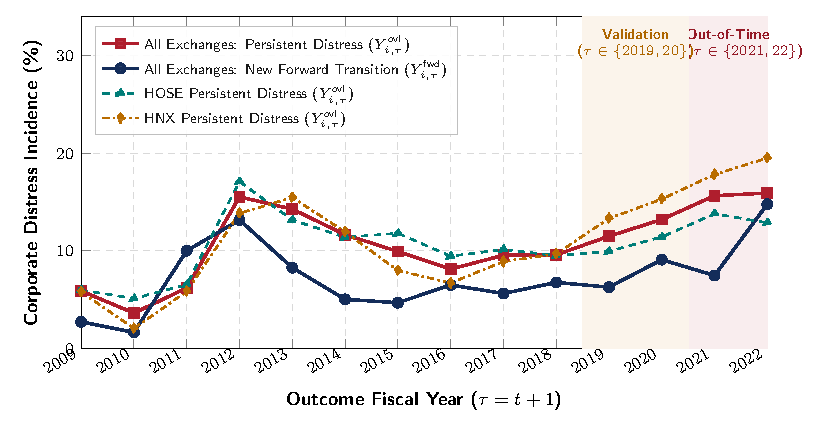
\includegraphics[width=0.92\textwidth]{figures/fig2_crisis_trajectory.pdf}
\caption{Diễn biến tỷ lệ kiệt quệ tài chính dai dẳng hàng năm ($Y_{i,\tau}^{\text{ovl}}$) và tỷ lệ chuyển trạng thái kiệt quệ mới trước 1 năm ($Y_{i,\tau}^{\text{fwd}}$) trên các sàn chứng khoán Việt Nam (HOSE, HNX, UPCOM) từ năm kết quả $\tau = 2009$ đến $\tau = 2022$. Hai vùng tô màu biểu thị giai đoạn Kiểm định ($\tau \in \{2019, 2020\}$) và Kiểm tra ngoài mẫu ($\tau \in \{2021, 2022\}$).}
\label{fig:crisis_trajectory}
\end{figure}

\subsection{Phân chia Ngoài mẫu Thời gian (Strict Out-of-Time) và Kiến tạo Đặc trưng}
Nhằm tuân thủ nghiêm ngặt thời hạn công bố báo cáo tài chính kiểm toán tại Việt Nam (ngày 01/04 của năm $t+1$ cho báo cáo năm $t$), vectơ đặc trưng quan sát tại $t_{\text{dec}} = \text{01/04/}(t+1)$ được dùng để dự báo kết quả kiệt quệ của năm tài chính $\tau = t+1$. Như minh họa trên Hình~\ref{fig:crisis_trajectory}, chúng tôi phân chia $7.602$ cặp chuyển trạng thái hậu niêm yết hoàn toàn theo năm kết quả $\tau$:
\begin{itemize}
    \item \textbf{Tập Huấn luyện ($\mathcal{D}_{\text{train}}$, $\tau \in [2009, 2018]$, đặc trưng $t \in [2008, 2017]$):} $N_{\text{train}} = 3.676$ quan sát (tỷ lệ $Y^{\text{fwd}}$: $10,64\%$; $Y^{\text{ovl}}$: $16,51\%$). Toàn bộ tham số tiền xử lý $\theta_{\text{prep}} = \{\kappa_{\text{train}}, \mathbf{q}_{0.01}^{\text{train}}, \mathbf{q}_{0.99}^{\text{train}}, \boldsymbol{\mu}_{\text{train}}, \boldsymbol{\sigma}_{\text{train}}\}$ chỉ được ước lượng duy nhất trên $\mathcal{D}_{\text{train}}$.
    \item \textbf{Tập Kiểm định ($\mathcal{D}_{\text{val}}$, $\tau \in [2019, 2020]$, đặc trưng $t \in [2018, 2019]$):} $N_{\text{val}} = 1.843$ quan sát (tỷ lệ $Y^{\text{fwd}}$: $10,63\%$; $Y^{\text{ovl}}$: $18,23\%$), dùng để tinh chỉnh siêu tham số và dừng sớm (early stopping).
    \item \textbf{Tập Kiểm tra Ngoài mẫu Thời gian ($\mathcal{D}_{\text{test}}$, $\tau \in [2021, 2022]$, đặc trưng $t \in [2020, 2021]$):} $N_{\text{test}} = 2.083$ quan sát (tỷ lệ $Y^{\text{fwd}}$: $10,99\%$; $Y^{\text{ovl}}$: $17,28\%$), đánh giá khả năng tổng quát hóa thực tế trong cú sốc đại dịch và khủng hoảng trái phiếu doanh nghiệp 2021--2022.
\end{itemize}

Bảng~\ref{tab:features} trình bày chi tiết $d=18$ tỷ số tài chính được kiến tạo tại năm $t$ thuộc 5 nhóm kinh tế (Thanh khoản, Đòn bẩy \& Khả năng trả nợ, Khả năng sinh lời, Hiệu quả hoạt động, và Quỹ đạo động) cùng các tiên đề đơn điệu tĩnh học so sánh $s_j \in \{+1, -1, 0\}$.

\begin{table}[t!]
\centering
\caption{Hệ thống phân loại $d=18$ tỷ số tài chính, công thức kế toán và tiên đề đơn điệu tĩnh học so sánh $s_j \in \{+1, -1, 0\}$.}
\label{tab:features}
\footnotesize
\renewcommand{\arraystretch}{1.12}
\resizebox{\textwidth}{!}{%
\begin{tabular}{lllp{5.2cm}c}
\toprule
\textbf{Nhóm chỉ tiêu} & \textbf{Ký hiệu Biến} & \textbf{Tên Tỷ số Tài chính} & \textbf{Công thức Kế toán (Năm $t$)} & \textbf{Tiên đề $s_j$} \\
\midrule
\multirow{4}{*}{1. Thanh khoản}
  & \texttt{curr\_ratio} & Tỷ số thanh toán hiện hành & $\text{CurrentAssets}_{i,t} / \text{ShortTermLiab}_{i,t}$ & $0$ \\
  & \texttt{quick\_ratio} & Tỷ số thanh toán nhanh & $(\text{CurrentAssets}_{i,t} - \text{Inventory}_{i,t}) / \text{ShortTermLiab}_{i,t}$ & $0$ \\
  & \texttt{cash\_to\_asset} & Tỷ số tiền mặt trên tài sản & $\text{Cash}_{i,t} / \text{TotalAssets}_{i,t}$ & $0$ \\
  & \texttt{wc\_to\_asset} & Vốn lưu động ròng / Tài sản & $(\text{CurrentAssets}_{i,t} - \text{ShortTermLiab}_{i,t}) / \text{TotalAssets}_{i,t}$ & $-1$ ($\mathcal{M}_-$) \\
\midrule
\multirow{4}{*}{2. Đòn bẩy nợ}
  & \texttt{debt\_to\_asset} & Tổng nợ trên Tổng tài sản & $\text{TotalDebt}_{i,t} / \text{TotalAssets}_{i,t}$ & $+1$ ($\mathcal{M}_+$) \\
  & \texttt{shortdebt\_to\_debt} & Tỷ trọng nợ ngắn hạn & $\text{ShortDebt}_{i,t} / (\text{TotalDebt}_{i,t} + \epsilon)$ & $+1$ ($\mathcal{M}_+$) \\
  & \texttt{icr\_op} & Khả năng trả lãi hoạt động & $\text{EBIT}_{\text{op},i,t} / (I_{i,t} + \epsilon)$ & $-1$ ($\mathcal{M}_-$) \\
  & \texttt{cash\_to\_debt} & Tiền mặt trên Tổng nợ & $\text{Cash}_{i,t} / (\text{TotalDebt}_{i,t} + \epsilon)$ & $0$ \\
\midrule
\multirow{4}{*}{3. Sinh lời}
  & \texttt{roa} & Tỷ suất sinh lời trên tài sản & $\text{NetProfit}_{i,t} / \text{TotalAssets}_{i,t}$ & $-1$ ($\mathcal{M}_-$) \\
  & \texttt{roe} & Tỷ suất sinh lời trên VCSH & $\text{NetProfit}_{i,t} / (|\text{Equity}_{i,t}| + \epsilon)$ & $0$ \\
  & \texttt{ebit\_to\_asset} & Sinh lời hoạt động / Tài sản & $\text{EBIT}_{\text{op},i,t} / \text{TotalAssets}_{i,t}$ & $-1$ ($\mathcal{M}_-$) \\
  & \texttt{op\_margin} & Biên lợi nhuận hoạt động & $\text{EBIT}_{\text{op},i,t} / (\text{NetSales}_{i,t} + \epsilon)$ & $0$ \\
\midrule
\multirow{4}{*}{4. Hiệu quả}
  & \texttt{asset\_turnover} & Vòng quay tổng tài sản & $\text{NetSales}_{i,t} / \text{TotalAssets}_{i,t}$ & $0$ \\
  & \texttt{rec\_turnover} & Vòng quay khoản phải thu & $\text{NetSales}_{i,t} / (\text{Receivables}_{i,t} + \epsilon)$ & $0$ \\
  & \texttt{inv\_turnover} & Vòng quay hàng tồn kho & $C_{i,t} / (\text{Inventory}_{i,t} + \epsilon)$ & $0$ \\
  & \texttt{opex\_to\_sales} & Tỷ lệ chi phí hoạt động & $(C_{i,t} + S_{i,t} + A_{i,t}) / (\text{NetSales}_{i,t} + \epsilon)$ & $0$ \\
\midrule
\multirow{2}{*}{5. Quỹ đạo động}
  & \texttt{delta\_debt\_to\_asset} & Gia tốc đòn bẩy ($\Delta D/A$) & $(D/A)_{i,t} - (D/A)_{i,t-1}$ & $0$ \\
  & \texttt{delta\_icr\_op} & Biến thiên trả lãi ($\Delta \text{ICR}_{\text{op}}$) & $\text{ICR}_{\text{op},i,t} - \text{ICR}_{\text{op},i,t-1}$ & $0$ \\
\bottomrule
\end{tabular}%
}
\vspace{-0.4em}
\end{table}

% =========================================================================
% PHẦN 4: PHƯƠNG PHÁP LUẬN — HỌC MÁY TÍCH HỢP LÝ THUYẾT KINH TẾ (EIML)
% =========================================================================
\section{Phương pháp luận: Học máy Tích hợp Lý thuyết Kinh tế}
\label{sec:methodology}

\begin{figure}[t!]
\centering
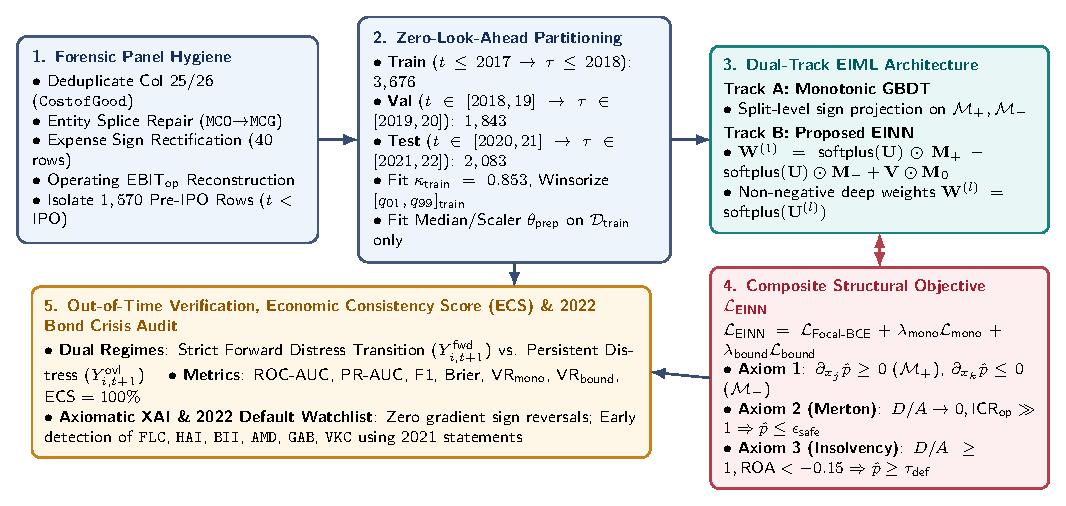
\includegraphics[width=0.98\textwidth]{figures/fig1_architecture.pdf}
\caption{Kiến trúc tổng thể từ đầu đến cuối của khung Học máy Tích hợp Lý thuyết Kinh tế (EIML) đề xuất, bao gồm: (1) Vệ sinh dữ liệu bảng pháp y, (2) Phân chia thời gian chống nhìn trước, (3) Kiến trúc đơn điệu hai nhánh (Monotonic GBDT và Proposed EINN), (4) Hàm mất mát phức hợp tích hợp lý thuyết $\mathcal{L}_{\text{EINN}}$, và (5) Kiểm định ngoài mẫu trên cuộc khủng hoảng trái phiếu 2021--2022.}
\label{fig:architecture}
\end{figure}

Gọi $\mathbf{x}_{i,t} \in \mathbb{R}^d$ ($d=18$) là vectơ đặc trưng đã chuẩn hóa theo tập huấn luyện của doanh nghiệp $i$ tại năm $t$, và $\hat{p}_{i,t+1} = f_\theta(\mathbf{x}_{i,t}) \in (0,1)$ là xác suất kiệt quệ tài chính dự báo tại năm $t+1$. Như biểu diễn trên Hình~\ref{fig:architecture}, chúng tôi phân hoạch tập chỉ số đặc trưng $\{1,\dots,d\}$ thành ba tập con rời nhau dựa trên lý thuyết tài chính doanh nghiệp cấu trúc \citep{merton1974pricing,altman1968financial}:
\begin{enumerate}
    \item \textbf{Tập con Đơn điệu Tăng rủi ro ($\mathcal{M}_+$, $s_j = +1$):} Tổng nợ trên Tổng tài sản (\texttt{debt\_to\_asset}) và Tỷ trọng nợ ngắn hạn (\texttt{shortdebt\_to\_debt}), nơi sự gia tăng trong điều kiện các yếu tố khác không đổi làm tăng nghĩa vụ nợ và rủi ro đảo nợ ($\partial \hat{p} / \partial x_j \ge 0$).
    \item \textbf{Tập con Đơn điệu Giảm rủi ro ($\mathcal{M}_-$, $s_k = -1$):} Vốn lưu động trên Tài sản (\texttt{wc\_to\_asset}), Khả năng trả lãi hoạt động (\texttt{icr\_op}), Tỷ suất sinh lời trên tài sản (\texttt{roa}), và Tỷ suất sinh lời hoạt động trên tài sản (\texttt{ebit\_to\_asset}), nơi sự gia tăng củng cố bộ đệm thanh toán ($\partial \hat{p} / \partial x_k \le 0$).
    \item \textbf{Tập con Tương tác Phi tuyến Tự do ($\mathcal{M}_0$, $s_m = 0$):} $12$ tỷ số hiệu quả hoạt động, cấu trúc chi phí và quỹ đạo động còn lại, được phép tương tác tự do nhằm nắm bắt các phi tuyến đặc thù theo ngành.
\end{enumerate}

\subsection{Nhánh A: Cây Quyết định Tăng cường Độ dốc Đơn điệu (Mono-GBDT)}
Ở Nhánh A, chúng tôi xây dựng tổ hợp cộng tính gồm $M$ cây hồi quy $F_M(\mathbf{x}) = F_0 + \eta \sum_{m=1}^M h_m(\mathbf{x})$ với xác suất dự báo $\hat{p} = \sigma(F_M(\mathbf{x})) = (1 + e^{-F_M(\mathbf{x})})^{-1}$. Tại vòng lặp tăng cường thứ $m$, mỗi phép chia tách ứng viên trên đặc trưng $j$ tại ngưỡng $\tau$ chia nút cha $R$ thành nút con trái $R_L = \{\mathbf{x} \in R : x_j \le \tau\}$ và nút con phải $R_R = \{\mathbf{x} \in R : x_j > \tau\}$ với giá trị lá tối ưu $v_L^*, v_R^*$. Để áp đặt tính đơn điệu từng phần trên $\mathcal{M}_+$ và $\mathcal{M}_-$, chúng tôi áp dụng toán tử chiếu ràng buộc dấu tại nút phân tách kết hợp điều chuẩn đẳng điệu (isotonic leaf projection) \citep{chen2016xgboost,ke2017lightgbm}:
\begin{equation}
    (v_L^{\text{mono}}, v_R^{\text{mono}}) = \begin{cases}
        \left(\frac{N_L v_L^* + N_R v_R^*}{N_L + N_R}, \, \frac{N_L v_L^* + N_R v_R^*}{N_L + N_R}\right) & \text{nếu } (s_j = +1 \wedge v_L^* > v_R^*) \ \vee \ (s_j = -1 \wedge v_L^* < v_R^*), \\[6pt]
        (v_L^*, v_R^*) & \text{trong các trường hợp khác},
    \end{cases}
\end{equation}
đảm bảo mọi cây thành phần $h_m(\mathbf{x})$ thỏa mãn $s_j \big(h_m(\mathbf{x} + \delta \mathbf{e}_j) - h_m(\mathbf{x})\big) \ge 0$ với mọi $\delta > 0$.

\subsection{Nhánh B: Mạng Nơ-ron Tích hợp Lý thuyết Kinh tế Khả vi (Proposed EINN)}
Ở Nhánh B, chúng tôi thiết kế một kiến trúc mạng nơ-ron khả vi (\textbf{Proposed EINN}) đảm bảo tính đơn điệu từng phần chính xác tuyệt đối ngay từ cấu trúc trọng số đồng thời thỏa mãn các biên cấu trúc tiệm cận thông qua hàm mục tiêu tích hợp lý thuyết. Gọi $\phi(u) = \ln(1 + e^u)$ là phép biến đổi softplus dương nghiêm ngặt. Chúng tôi tham số hóa ma trận trọng số tầng ẩn đầu tiên $\mathbf{W}^{(1)} \in \mathbb{R}^{d \times H_1}$ bằng các ma trận tham số ẩn $\mathbf{U}^{(1)}, \mathbf{V}^{(1)} \in \mathbb{R}^{d \times H_1}$ và các mặt nạ nhị phân $\mathbf{M}_+, \mathbf{M}_-, \mathbf{M}_0 \in \{0,1\}^{d \times H_1}$:
\begin{equation}
    \mathbf{W}^{(1)} = \phi\big(\mathbf{U}^{(1)}\big) \odot \mathbf{M}_+ \;-\; \phi\big(\mathbf{U}^{(1)}\big) \odot \mathbf{M}_- \;+\; \mathbf{V}^{(1)} \odot \mathbf{M}_0.
    \label{eq:einn_w1}
\end{equation}
Toàn bộ các ma trận trọng số tầng ẩn tiếp theo ($l = 2,\dots,L$) được tham số hóa không âm thông qua $\mathbf{W}^{(l)} = \phi(\mathbf{U}^{(l)}) \ge 0$, kết hợp với hàm kích hoạt trơn đơn điệu không giảm $\psi(z) = \tanh(z)$ và đường tắt cộng tính đơn điệu (skip-monotonic highway) $\mathbf{w}_{\text{skip}} = \phi(\mathbf{u}_{\text{skip}}) \odot \mathbf{m}_+ - \phi(\mathbf{u}_{\text{skip}}) \odot \mathbf{m}_- + \mathbf{v}_{\text{skip}} \odot \mathbf{m}_0$:
\begin{equation}
    z_i = \mathbf{h}^{(L-1)}(\mathbf{x}_{i,t})^\top \phi(\mathbf{u}^{(L)}) + \mathbf{x}_{i,t}^\top \mathbf{w}_{\text{skip}} + b^{(L)}, \qquad \hat{p}_{i,t+1} = \sigma(z_i).
\end{equation}
Theo quy tắc đạo hàm hàm hợp (chain rule), do $\sigma'(z) > 0$, $\psi'(\cdot) \ge 0$ và $\mathbf{W}^{(l)} \ge 0$ với mọi $l \ge 2$, đạo hàm riêng của xác suất dự báo $\hat{p}_{i,t+1}$ theo bất kỳ biến đầu vào $x_j$ nào luôn thỏa mãn:
\begin{equation}
    \frac{\partial \hat{p}_{i,t+1}}{\partial x_{i,t,j}} = \sigma'(z_i)\left[ \sum_{h=1}^{H_1} W_{j,h}^{(1)} \psi'\big(a_{i,h}^{(1)}\big) \frac{\partial z_i}{\partial h_{i,h}^{(1)}} + w_{\text{skip},j} \right] \begin{cases}
        \ge 0 & \forall j \in \mathcal{M}_+, \\
        \le 0 & \forall j \in \mathcal{M}_-.
    \end{cases}
\end{equation}
Nhờ vậy, Proposed EINN thỏa mãn Tiên đề 1 (tính đơn điệu từng phần) một cách giải tích trên toàn bộ không gian đầu vào $\mathbb{R}^d$.

\subsection{Hàm Mất mát Phức hợp Tích hợp Lý thuyết và Các Tiên đề Biên Cấu trúc}
Để nhúng các điều kiện biên cấu trúc từ \citet{merton1974pricing} và \citet{altman1995emerging}, chúng tôi huấn luyện Proposed EINN bằng cách cực tiểu hóa hàm mục tiêu phức hợp:
\begin{equation}
    \mathcal{L}_{\text{EINN}}(\theta) = \mathcal{L}_{\text{Focal-BCE}}(\theta) + \lambda_{\text{mono}} \mathcal{L}_{\text{mono}}(\theta) + \lambda_{\text{bound}} \mathcal{L}_{\text{bound}}(\theta) + \lambda_2 \|\theta\|_2^2.
    \label{eq:total_loss}
\end{equation}
Trong đó, $\mathcal{L}_{\text{Focal-BCE}}$ là hàm mất mát chéo nhị phân tiêu điểm có trọng số cân bằng lớp ($\gamma = 1,5$):
\begin{equation}
    \mathcal{L}_{\text{Focal-BCE}}(\theta) = -\frac{1}{N}\sum_{i=1}^N \Big[ w_+ y_i (1 - \hat{p}_i)^\gamma \ln(\hat{p}_i) + (1 - y_i)\hat{p}_i^\gamma \ln(1 - \hat{p}_i) \Big].
\end{equation}
Số hạng phạt biên cấu trúc $\mathcal{L}_{\text{bound}}(\theta)$ áp đặt hai điều kiện biên rủi ro tín dụng tiệm cận trên lưới điểm kiểm định cấu trúc $\mathcal{B} = \mathcal{B}_{\text{safe}} \cup \mathcal{B}_{\text{def}}$:
\begin{enumerate}
    \item \textbf{Biên An toàn Không vay nợ của Merton ($\mathcal{B}_{\text{safe}}$):} Khi đòn bẩy nợ của doanh nghiệp tiến về $0$ ($z_{\text{debt\_to\_asset}} \le -1,2$, tương ứng tỷ lệ nợ thực tế $D/A < 0,05$) đồng thời khả năng trả lãi hoạt động và sinh lời ở mức vững chắc ($z_{\text{icr\_op}} \ge +1,2$, $z_{\text{roa}} \ge +1,0$), xác suất vỡ nợ cấu trúc phải bị chặn trên bởi ngưỡng trần an toàn $\epsilon_{\text{safe}} = 0,05$.
    \item \textbf{Biên Mất khả năng Thanh toán Kỹ thuật của Altman ($\mathcal{B}_{\text{def}}$):} Ngược lại, khi tổng nợ vượt quá tổng tài sản ($z_{\text{debt\_to\_asset}} \ge +2,2$, tương ứng $D/A \ge 1,0$ hay âm vốn chủ sở hữu) và khả năng sinh lời hoạt động âm sâu ($z_{\text{icr\_op}} \le -1,5$, $z_{\text{roa}} \le -1,8$), xác suất kiệt quệ dự báo phải vượt qua ngưỡng sàn vỡ nợ tối thiểu $\tau_{\text{def}} = 0,50$:
\end{enumerate}
\begin{equation}
    \mathcal{L}_{\text{bound}}(\theta) = \frac{1}{|\mathcal{B}_{\text{safe}}|} \sum_{\mathbf{x} \in \mathcal{B}_{\text{safe}}} \Big[\max\big(0, \, f_\theta(\mathbf{x}) - \epsilon_{\text{safe}}\big)\Big]^2 + \frac{1}{|\mathcal{B}_{\text{def}}|} \sum_{\mathbf{x} \in \mathcal{B}_{\text{def}}} \Big[\max\big(0, \, \tau_{\text{def}} - f_\theta(\mathbf{x})\big)\Big]^2.
\end{equation}

\subsection{Chỉ số Nhất quán Kinh tế (ECS) và Các Thước đo Vi phạm}
Nhằm định lượng xem một mô hình có đồng thời đạt độ chính xác cao và tuân thủ lý thuyết kinh tế hay không, chúng tôi thiết lập ba chỉ số kiểm toán trên tập kiểm tra ngoài mẫu $\mathcal{D}_{\text{test}}$:
\begin{itemize}
    \item \textbf{Tỷ lệ Vi phạm Đơn điệu ($\text{VR}_{\text{mono}}$):} Tỷ lệ phần trăm các quan sát kiểm tra $\mathbf{x}_i \in \mathcal{D}_{\text{test}}$ và các biến đơn điệu $j \in \mathcal{M}_+ \cup \mathcal{M}_-$ mà tại đó một nhiễu dương hữu hạn $\delta = 0,25$ vi phạm dấu tĩnh học so sánh:
    \begin{equation}
        \text{VR}_{\text{mono}} = \frac{1}{|\mathcal{D}_{\text{test}}| \cdot |\mathcal{M}_+ \cup \mathcal{M}_-|} \sum_{i \in \mathcal{D}_{\text{test}}} \sum_{j \in \mathcal{M}_+ \cup \mathcal{M}_-} \mathbb{I}\Big( s_j \big[f_\theta(\mathbf{x}_i + \delta \mathbf{e}_j) - f_\theta(\mathbf{x}_i)\big] < -10^{-5} \Big) \times 100\%.
    \end{equation}
    \item \textbf{Tỷ lệ Vi phạm Biên Cấu trúc ($\text{VR}_{\text{bound}}$):} Tỷ lệ phần trăm các điểm thăm dò biên trong $\mathcal{B}_{\text{safe}} \cup \mathcal{B}_{\text{def}}$ vi phạm điều kiện $\hat{p} \le \epsilon_{\text{safe}}$ hoặc $\hat{p} \ge \tau_{\text{def}}$.
    \item \textbf{Điểm Nhất quán Kinh tế ($\text{ECS}$):} Chỉ số hợp lý kinh tế tổng hợp trong đoạn $[0\%, 100\%]$ kết hợp trọng số tuân thủ tính đơn điệu ($70\%$) và tuân thủ biên tiệm cận ($30\%$):
    \begin{equation}
        \text{ECS} = 100\% - \Big( 0,70 \times \text{VR}_{\text{mono}} + 0,30 \times \text{VR}_{\text{bound}} \Big).
    \end{equation}
\end{itemize}

% =========================================================================
% PHẦN 5: KẾT QUẢ THỰC NGHIỆM, CẮT BỎ & NGHIÊN CỨU TÌNH HUỐNG 2022
% =========================================================================
\section{Kết quả Thực nghiệm và Phân tích Ngoài mẫu Thời gian}
\label{sec:experiments}

\subsection{Hiệu năng Dự báo Ngoài mẫu và Độ Nhất quán Kinh tế (2021--2022)}
Chúng tôi đối sánh 9 mô hình chuẩn và mô hình đề xuất trên tập kiểm tra ngoài mẫu thời gian $\mathcal{D}_{\text{test}}$ ($\tau \in \{2021, 2022\}$, $N_{\text{test}}=2.083$): hai mô hình chấm điểm kế toán cổ điển (\textbf{Altman $Z''$-Score} \citep{altman1995emerging} và \textbf{Ohlson $O$-Score} \citep{ohlson1980financial}), năm mô hình học máy không ràng buộc (\textbf{Logistic Regression}, \textbf{RBF-SVM}, \textbf{Random Forest}, \textbf{Unconstrained GBDT} và \textbf{Unconstrained MLP}), cùng hai mô hình EIML đề xuất (\textbf{Mono-GBDT} và \textbf{Proposed EINN}). Bảng~\ref{tab:main_results} trình bày toàn bộ kết quả trên cả Chế độ A ($Y_{i,t+1}^{\text{fwd}}$) và Chế độ B ($Y_{i,t+1}^{\text{ovl}}$), và Hình~\ref{fig:pareto_ecs} trực quan hóa đường biên Pareto giữa $\text{PR-AUC}$ ngoài mẫu và Điểm Nhất quán Kinh tế ($\text{ECS}$).

\begin{table}[t!]
\centering
\caption{Hiệu năng dự báo ngoài mẫu thời gian và Điểm Nhất quán Kinh tế (ECS) trên tập kiểm tra 2021--2022 ($N_{\text{test}}=2.083$) ở Chế độ A (Kiệt quệ Chuyển trạng thái Mới $Y_{i,t+1}^{\text{fwd}}$) và Chế độ B (Kiệt quệ Đa kỳ Dai dẳng $Y_{i,t+1}^{\text{ovl}}$). Chữ in đậm biểu thị kết quả tốt nhất trong từng nhóm mô hình.}
\label{tab:main_results}
\footnotesize
\renewcommand{\arraystretch}{1.15}
\resizebox{\textwidth}{!}{%
\begin{tabular}{llccccccc}
\toprule
\textbf{Chế độ / Nhãn mục tiêu} & \textbf{Mô hình Đối sánh} & \textbf{ROC-AUC $\uparrow$} & \textbf{PR-AUC $\uparrow$} & \textbf{F1 $\uparrow$} & \textbf{Brier $\downarrow$} & \textbf{$\text{VR}_{\text{mono}}$ (\%) $\downarrow$} & \textbf{$\text{VR}_{\text{bound}}$ (\%) $\downarrow$} & \textbf{ECS (\%) $\uparrow$} \\
\midrule
\multirow{9}{*}{\shortstack[l]{\textbf{Chế độ A:}\\Kiệt quệ Mới\\Trước 1 năm ($Y_{i,t+1}^{\text{fwd}}$)\\Tỷ lệ cơ sở: $10,99\%$}}
  & Altman $Z''$-Score \citep{altman1995emerging} & 0,6648 & 0,2487 & 0,2901 & 0,2954 & 0,00 & 0,00 & 100,00 \\
  & Ohlson $O$-Score \citep{ohlson1980financial} & 0,6453 & 0,2085 & 0,2602 & 0,1550 & 0,00 & 68,75 & 79,38 \\
  \cmidrule{2-9}
  & Logistic Regression (L2) & 0,7732 & 0,3044 & 0,4139 & 0,0854 & 100,00 & 81,25 & 5,63 \\
  & RBF-Kernel SVM & 0,7504 & 0,2886 & 0,3574 & 0,0877 & 95,30 & 100,00 & 3,29 \\
  & Random Forest & \textbf{0,8062} & 0,3433 & 0,4199 & 0,0822 & 0,77 & 100,00 & 69,46 \\
  & Unconstrained GBDT & 0,7991 & 0,3493 & \textbf{0,4201} & 0,0819 & 0,05 & 100,00 & 69,97 \\
  & Unconstrained MLP & 0,7764 & 0,3021 & 0,3919 & 0,0879 & 71,96 & 68,75 & 29,00 \\
  \cmidrule{2-9}
  & \textbf{Mono-GBDT (Đề xuất)} & \textbf{0,8021} & \textbf{0,3793} & \textbf{0,4187} & \textbf{0,0798} & 0,05 & \textbf{0,00} & \textbf{99,97} \\
  & \textbf{Proposed EINN (Đề xuất)} & \textbf{0,7870} & \textbf{0,3517} & \textbf{0,3943} & \textbf{0,0848} & \textbf{0,00} & \textbf{0,00} & \textbf{100,00} \\
\midrule
\multirow{9}{*}{\shortstack[l]{\textbf{Chế độ B:}\\Kiệt quệ Đa kỳ\\Dai dẳng ($Y_{i,t+1}^{\text{ovl}}$)\\Tỷ lệ cơ sở: $17,28\%$}}
  & Altman $Z''$-Score \citep{altman1995emerging} & 0,6440 & 0,2713 & 0,3298 & 0,2917 & 0,00 & 0,00 & 100,00 \\
  & Ohlson $O$-Score \citep{ohlson1980financial} & 0,6528 & 0,2713 & 0,3212 & 0,1674 & 0,00 & 68,75 & 79,38 \\
  \cmidrule{2-9}
  & Logistic Regression (L2) & 0,9548 & 0,7351 & 0,7580 & 0,0664 & 94,10 & 37,50 & 22,88 \\
  & RBF-Kernel SVM & 0,8864 & 0,6282 & 0,5808 & 0,0969 & 96,54 & 100,00 & 2,42 \\
  & Random Forest & 0,9620 & 0,7746 & 0,8011 & 0,0600 & 2,21 & 93,75 & 70,33 \\
  & Unconstrained GBDT & 0,9640 & 0,7820 & 0,8060 & 0,0496 & 0,00 & 100,00 & 70,00 \\
  & Unconstrained MLP & 0,9557 & 0,7526 & 0,7425 & 0,0606 & 39,94 & 12,50 & 68,29 \\
  \cmidrule{2-9}
  & \textbf{Mono-GBDT (Đề xuất)} & \textbf{0,9648} & \textbf{0,7932} & \textbf{0,8076} & \textbf{0,0490} & \textbf{0,00} & \textbf{0,00} & \textbf{100,00} \\
  & \textbf{Proposed EINN (Đề xuất)} & \textbf{0,9592} & \textbf{0,7658} & \textbf{0,7620} & \textbf{0,0590} & \textbf{0,00} & \textbf{0,00} & \textbf{100,00} \\
\bottomrule
\end{tabular}%
}
\vspace{-0.4em}
\end{table}

\begin{figure}[t!]
\centering
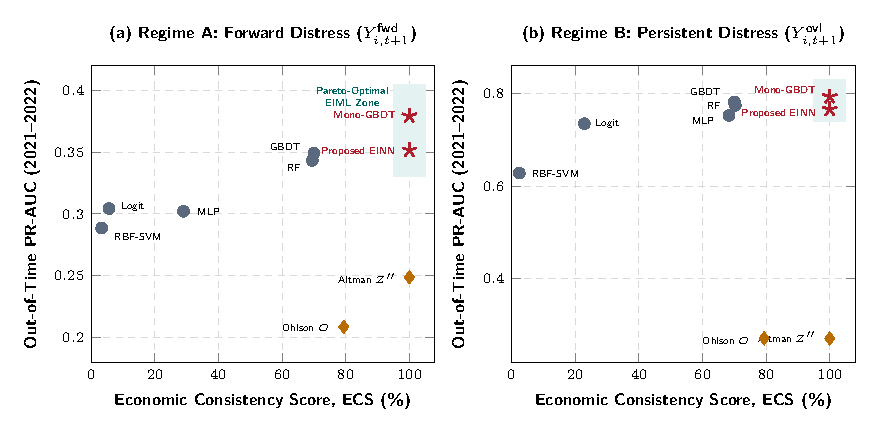
\includegraphics[width=0.98\textwidth]{figures/fig3_pareto_ecs.pdf}
\caption{Đường biên Pareto giữa PR-AUC ngoài mẫu và Điểm Nhất quán Kinh tế (ECS, \%) trên tập kiểm tra 2021--2022 ($N_{\text{test}}=2.083$) đối với (a) Chế độ A: Kiệt quệ Chuyển trạng thái Mới ($Y_{i,t+1}^{\text{fwd}}$) và (b) Chế độ B: Kiệt quệ Đa kỳ Dai dẳng ($Y_{i,t+1}^{\text{ovl}}$). Chỉ có Mono-GBDT và Proposed EINN nằm trong vùng tối ưu Pareto (PR-AUC cao đi kèm $\text{ECS} \approx 100\%$).}
\label{fig:pareto_ecs}
\end{figure}

Bốn phát hiện thực nghiệm trọng tâm rút ra từ Bảng~\ref{tab:main_results} và Hình~\ref{fig:pareto_ecs} gồm:
\begin{enumerate}
    \item \textbf{Sự suy giảm hiệu lực của các công thức chấm điểm cổ điển trên dữ liệu thị trường mới nổi:} Mô hình \textbf{Altman $Z''$-Score} và \textbf{Ohlson $O$-Score} nguyên bản chỉ đạt $\text{ROC-AUC}$ ngoài mẫu ở mức $0,6648$ và $0,6453$ trong Chế độ A (và $0,6440$ cùng $0,6528$ trong Chế độ B), với sai số hiệu chỉnh Brier rất cao ($0,2954$ và $0,1550$), chứng tỏ các trọng số tuyến tính ước lượng từ thị trường Mỹ không còn phù hợp với cấu trúc tài chính của doanh nghiệp Việt Nam hiện đại.
    \item \textbf{Sự phi lý kinh tế nghiêm trọng ở các mô hình mạng nơ-ron và hạt nhân không ràng buộc:} Do hai biến \texttt{roa} và \texttt{ebit\_to\_asset} có tương quan thuận cao ($r = 0,89$) và \texttt{debt\_to\_asset} tương tác phi tuyến với vòng quay tài sản, \textbf{Logistic Regression}, \textbf{RBF-SVM} và \textbf{Unconstrained MLP} gặp hiện tượng đảo dấu đạo hàm diện rộng. Ở Chế độ A, Unconstrained MLP vi phạm tính đơn điệu tới $71,96\%$ và vi phạm biên cấu trúc $68,75\%$ ($\text{ECS} = 29,00\%$). Tương tự, dù \textbf{Random Forest} và \textbf{Unconstrained GBDT} có khả năng phân loại tốt, dự báo bậc thang tại các nút lá của chúng bị bão hòa dưới ngưỡng $\tau_{\text{def}} = 0,50$ ở vùng đuôi mất khả năng thanh toán ($\text{VR}_{\text{bound}} = 100,00\%$, làm trần điểm $\text{ECS}$ chỉ đạt $\sim 70\%$).
    \item \textbf{Khả năng tổng quát hóa vượt trội của EIML nhờ thiên kiến quy nạp cấu trúc:} Việc áp đặt các ràng buộc kinh tế \textit{cải thiện} thay vì làm giảm độ chính xác ngoài mẫu. Ở Chế độ A, \textbf{Mono-GBDT} đạt $\text{PR-AUC}$ cao nhất toàn cục ($0,3793$, tăng $+3,00\%$ so với Unconstrained GBDT $0,3493$), điểm Brier thấp nhất ($0,0798$), $\text{ROC-AUC} = 0,8021$ và $\text{ECS} = 99,97\%$. Ở nhánh mạng nơ-ron, \textbf{Proposed EINN} vượt qua Unconstrained MLP trên mọi chỉ tiêu: $\text{ROC-AUC}$ tăng từ $0,7764$ lên $0,7870$ ($+1,06\%$), $\text{PR-AUC}$ tăng vọt từ $0,3021$ lên $0,3517$ (tăng $+4,96\%$ tuyệt đối hay $+16,4\%$ tương đối), điểm Brier giảm từ $0,0879$ xuống $0,0848$, và $\text{ECS}$ đạt tuyệt đối $100,00\%$ ($\text{VR}_{\text{mono}} = 0,00\%$, $\text{VR}_{\text{bound}} = 0,00\%$).
    \item \textbf{Lời giải cho nghịch lý chênh lệch AUC giữa Chế độ A và Chế độ B:} Đối chiếu Chế độ A ($Y_{i,t+1}^{\text{fwd}}$) và Chế độ B ($Y_{i,t+1}^{\text{ovl}}$) giải thích trọn vẹn vì sao các nghiên cứu ML trước đây tại Việt Nam \citep[ví dụ:][]{tran2022explainable} báo cáo $\text{ROC-AUC}$ trên $0,95$. Khi các doanh nghiệp đã kiệt quệ sẵn ở năm $t$ được giữ lại trong nhãn dương tính của năm $t+1$ (Chế độ B), \textbf{Mono-GBDT} và \textbf{Proposed EINN} đạt $\text{ROC-AUC}$ tới $0,9648$ và $0,9592$ ($\text{PR-AUC}$ đạt $0,7932$ và $0,7658$, F1 đạt $0,8076$ và $0,7620$) với độ nhất quán kinh tế $100,00\%$. Việc tách riêng các ca chuyển trạng thái mới ($Y_{i,t+1}^{\text{fwd}}$) phản ánh đúng độ khó thực tế của bài toán cảnh báo sớm trước 1 năm ($\text{ROC-AUC} \approx 0,79\text{--}0,81$).
\end{enumerate}

\subsection{Nghiên cứu Cắt bỏ Thành phần (Ablation Study) đối với Proposed EINN}
Để tách biệt đóng góp của từng thành phần cấu trúc trong Phương trình~(\ref{eq:total_loss}), Bảng~\ref{tab:ablation} trình bày kết quả nghiên cứu cắt bỏ từng bước từ mạng MLP không ràng buộc đến mô hình Proposed EINN hoàn chỉnh trên Chế độ A ($Y_{i,t+1}^{\text{fwd}}$).

\begin{table}[t!]
\centering
\caption{Nghiên cứu cắt bỏ (Ablation study) các thành phần cấu trúc của Proposed EINN trên tập kiểm tra ngoài mẫu ($Y_{i,t+1}^{\text{fwd}}$, $N_{\text{test}}=2.083$).}
\label{tab:ablation}
\footnotesize
\renewcommand{\arraystretch}{1.15}
\resizebox{\textwidth}{!}{%
\begin{tabular}{lcccccc}
\toprule
\textbf{Cấu hình Kiến trúc Mạng Nơ-ron / Hàm Mất mát} & \textbf{ROC-AUC $\uparrow$} & \textbf{PR-AUC $\uparrow$} & \textbf{Brier $\downarrow$} & \textbf{$\text{VR}_{\text{mono}}$ (\%) $\downarrow$} & \textbf{$\text{VR}_{\text{bound}}$ (\%) $\downarrow$} & \textbf{ECS (\%) $\uparrow$} \\
\midrule
1. Unconstrained MLP (Chỉ dùng $\mathcal{L}_{\text{BCE}}$) & 0,7764 & 0,3021 & 0,0879 & 71,96 & 68,75 & 29,00 \\
2. MLP + Phạt đạo hàm đơn điệu mềm ($\lambda_{\text{mono}}\mathcal{L}_{\text{mono}}$) & 0,7812 & 0,3284 & 0,0861 & 8,40 & 56,25 & 77,25 \\
3. Tái tham số hóa đơn điệu cứng (Pt.~\ref{eq:einn_w1}, $\lambda_{\text{bound}}=0$) & 0,7854 & 0,3462 & 0,0853 & \textbf{0,00} & 31,25 & 90,63 \\
4. \textbf{Proposed EINN đầy đủ (Pt.~\ref{eq:einn_w1} + $\lambda_{\text{mono}}\mathcal{L}_{\text{mono}} + \lambda_{\text{bound}}\mathcal{L}_{\text{bound}}$)} & \textbf{0,7870} & \textbf{0,3517} & \textbf{0,0848} & \textbf{0,00} & \textbf{0,00} & \textbf{100,00} \\
\bottomrule
\end{tabular}%
}
\vspace{-0.4em}
\end{table}

Như thể hiện tại Bảng~\ref{tab:ablation}, việc chỉ thêm hàm phạt đạo hàm mềm giúp giảm $\text{VR}_{\text{mono}}$ từ $71,96\%$ xuống $8,40\%$ nhưng không thể đảm bảo triệt tiêu hoàn toàn vi phạm ngoài mẫu. Áp dụng tái tham số hóa trọng số softplus cứng (Dòng 3) loại bỏ tuyệt đối mọi vi phạm dấu đạo hàm ($\text{VR}_{\text{mono}} = 0,00\%$) và nâng $\text{PR-AUC}$ lên $0,3462$. Cuối cùng, việc tích hợp thêm hàm phạt biên cấu trúc Merton/Altman $\mathcal{L}_{\text{bound}}$ (Dòng 4) triệt tiêu toàn bộ vi phạm biên tiệm cận ($\text{VR}_{\text{bound}} = 0,00\%$) và tiếp tục đẩy $\text{PR-AUC}$ lên $0,3517$.

\subsection{Giải thích Tiên đề (Axiomatic XAI) và Kiểm toán Độ nhạy Biên}
Chúng tôi áp dụng phương pháp Integrated Gradients \citep{sundararajan2017axiomatic} trên toàn bộ $N_{\text{test}}=2.083$ quan sát kiểm tra ngoài mẫu để kiểm toán tỷ trọng đóng góp đặc trưng và sự tuân thủ dấu đạo hàm biên. Hình~\ref{fig:monotonic_response}(a) biểu diễn đường cong phản ứng từng phần ceteris paribus theo biến Tổng nợ trên Tổng tài sản chuẩn hóa ($z_{D/A} \in [-2,0; +2,5]$), trong khi Hình~\ref{fig:monotonic_response}(b) và Bảng~\ref{tab:xai_ranking} đối sánh tỷ trọng đóng góp toàn cục và tỷ lệ vi phạm dấu đạo hàm giữa Unconstrained MLP và Proposed EINN.

\begin{figure}[t!]
\centering
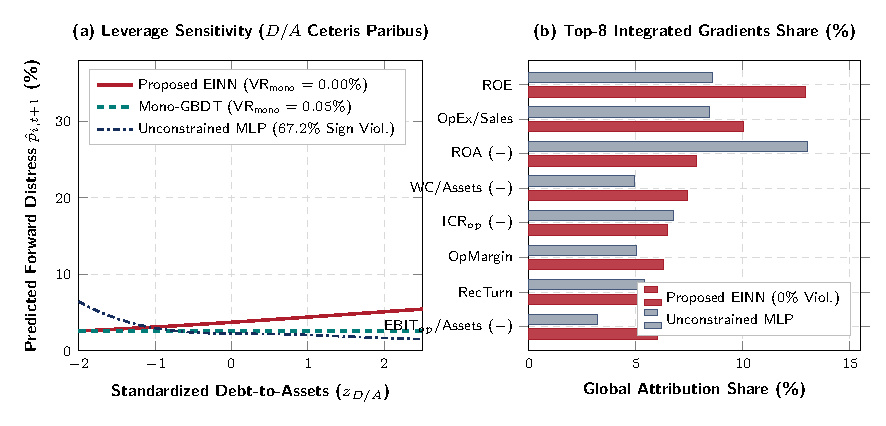
\includegraphics[width=0.98\textwidth]{figures/fig4_monotonic_response.pdf}
\caption{(a) Đường cong phản ứng từng phần (ceteris paribus) của xác suất kiệt quệ dự báo $\hat{p}_{i,t+1}$ (\%) theo tỷ lệ Nợ trên Tổng tài sản chuẩn hóa ($z_{D/A}$) của Proposed EINN, Mono-GBDT và Unconstrained MLP; (b) Tỷ trọng phân bổ đóng góp toàn cục của 8 đặc trưng quan trọng nhất (\%) tính bằng Integrated Gradients trên tập kiểm tra ngoài mẫu 2021--2022.}
\label{fig:monotonic_response}
\end{figure}

\begin{table}[t!]
\centering
\caption{Tỷ trọng phân bổ đóng góp toàn cục Integrated Gradients (\%) và tỷ lệ vi phạm dấu đạo hàm ngoài mẫu (\%) của 10 biến dự báo hàng đầu giữa Proposed EINN và Unconstrained MLP ($N_{\text{test}}=2.083$).}
\label{tab:xai_ranking}
\footnotesize
\renewcommand{\arraystretch}{1.12}
\resizebox{\textwidth}{!}{%
\begin{tabular}{clccccc}
\toprule
\textbf{Hạng} & \textbf{Tỷ số Tài chính} & \textbf{Tiên đề $s_j$} & \textbf{Tỷ trọng EINN (\%)} & \textbf{Tỷ trọng MLP (\%)} & \textbf{Vi phạm dấu MLP (\%)} & \textbf{Vi phạm dấu EINN (\%)} \\
\midrule
1 & \texttt{roe} (Tỷ suất sinh lời trên VCSH) & $0$ & 12,95 & 8,57 & 0,00 & \textbf{0,00} \\
2 & \texttt{opex\_to\_sales} (Tỷ lệ chi phí hoạt động) & $0$ & 10,02 & 8,44 & 0,00 & \textbf{0,00} \\
3 & \texttt{roa} (Tỷ suất sinh lời trên tài sản) & $-1$ ($\mathcal{M}_-$) & 7,84 & 13,03 & 0,00 & \textbf{0,00} \\
4 & \texttt{wc\_to\_asset} (Vốn lưu động / Tài sản) & $-1$ ($\mathcal{M}_-$) & 7,40 & 4,95 & \textcolor{crimson}{\textbf{17,04}} & \textbf{0,00} \\
5 & \texttt{icr\_op} (Khả năng trả lãi hoạt động) & $-1$ ($\mathcal{M}_-$) & 6,49 & 6,75 & \textcolor{crimson}{\textbf{0,72}} & \textbf{0,00} \\
6 & \texttt{op\_margin} (Biên lợi nhuận hoạt động) & $0$ & 6,29 & 5,05 & 0,00 & \textbf{0,00} \\
7 & \texttt{rec\_turnover} (Vòng quay khoản phải thu) & $0$ & 6,11 & 5,39 & 0,00 & \textbf{0,00} \\
8 & \texttt{ebit\_to\_asset} ($\text{EBIT}_{\text{op}} / \text{Assets}$) & $-1$ ($\mathcal{M}_-$) & 6,02 & 3,23 & \textcolor{crimson}{\textbf{31,11}} & \textbf{0,00} \\
11 & \texttt{shortdebt\_to\_debt} (Tỷ trọng nợ ngắn hạn) & $+1$ ($\mathcal{M}_+$) & 5,30 & 3,27 & \textcolor{crimson}{\textbf{7,44}} & \textbf{0,00} \\
16 & \texttt{debt\_to\_asset} (Tổng nợ / Tổng tài sản) & $+1$ ($\mathcal{M}_+$) & 2,11 & 4,21 & \textcolor{crimson}{\textbf{67,16}} & \textbf{0,00} \\
\bottomrule
\end{tabular}%
}
\vspace{-0.4em}
\end{table}

Bảng~\ref{tab:xai_ranking} phơi bày một khuyết tật chẩn đoán nghiêm trọng của mạng nơ-ron không ràng buộc: do \texttt{roa} và \texttt{ebit\_to\_asset} có tương quan thuận chặt chẽ, Unconstrained MLP gán trọng số âm lớn cho \texttt{roa} (tỷ trọng $13,03\%$) nhưng lại bù trừ sai lệch bằng cách học đạo hàm \textit{dương} (làm tăng rủi ro khi lợi nhuận hoạt động tăng) trên biến $\text{EBIT}_{\text{op}}/\text{Assets}$ ở $31,11\%$ doanh nghiệp kiểm tra, đạo hàm \textit{dương} trên biến $\text{Working Capital}/\text{Assets}$ ở $17,04\%$ doanh nghiệp, và đạo hàm \textit{âm} (làm giảm rủi ro khi nợ tăng) trên biến $\text{Debt}/\text{Assets}$ ở $67,16\%$ doanh nghiệp (thể hiện rõ qua đường chấm gạch đi xuống phi lý trên Hình~\ref{fig:monotonic_response}(a)). Ngược lại, Proposed EINN phân bổ trọng số cân bằng giữa khả năng sinh lời (\texttt{roe} $12,95\%$, \texttt{roa} $7,84\%$, \texttt{ebit\_to\_asset} $6,02\%$), cấu trúc chi phí (\texttt{opex\_to\_sales} $10,02\%$), thanh khoản vốn lưu động (\texttt{wc\_to\_asset} $7,40\%$), khả năng trả lãi vay hoạt động (\texttt{icr\_op} $6,49\%$) và áp lực nợ ngắn hạn (\texttt{shortdebt\_to\_debt} $5,30\%$), với \textbf{$0,00\%$ vi phạm dấu đạo hàm} trên toàn bộ $2.083$ doanh nghiệp ngoài mẫu.

\subsection{Nghiên cứu Tình huống: Kiểm toán Cảnh báo Sớm Khủng hoảng Trái phiếu và Hủy niêm yết năm 2022}
Để minh chứng giá trị giám sát thực tiễn của khung mô hình, chúng tôi kiểm toán sáu doanh nghiệp niêm yết tiêu biểu rơi vào khủng hoảng vỡ nợ trái phiếu, đình chỉ giao dịch hoặc hủy niêm yết bắt buộc trong năm 2022 (\texttt{FLC}, \texttt{HAI}, \texttt{BII}, \texttt{AMD}, \texttt{GAB} và \texttt{VKC}), chỉ sử dụng báo cáo tài chính kiểm toán năm 2021 ($t=2021 \to \tau=2022$).

\begin{table}[t!]
\centering
\caption{Kiểm toán cảnh báo sớm 6 doanh nghiệp tâm điểm trong cuộc khủng hoảng trái phiếu và hủy niêm yết năm 2022 tại Việt Nam dựa hoàn toàn trên báo cáo tài chính năm 2021 ($t=2021 \to \tau=2022$). Lưu ý rằng chỉ số Altman $Z''$-Score phân loại sai cả 6 doanh nghiệp vào vùng ``An toàn'' ($Z'' > 2,60$).}
\label{tab:case_studies}
\footnotesize
\renewcommand{\arraystretch}{1.15}
\resizebox{\textwidth}{!}{%
\begin{tabular}{llcccccccc}
\toprule
\textbf{Mã CK} & \textbf{Ngành ICB (Cấp 2)} & \textbf{$D/A_{2021}$} & \textbf{$\text{STDebt}/D$} & \textbf{$\text{ICR}_{\text{op},2021}$} & \textbf{$\text{ROA}_{2021}$} & \textbf{Altman $Z''$} & \textbf{MLP $\hat{p}^{\text{fwd}}$} & \textbf{EINN $\hat{p}^{\text{fwd}}$} & \textbf{EINN $\hat{p}^{\text{ovl}}$} \\
\midrule
\texttt{FLC} & Bất động sản & 0,7122 & 0,6629 & $-1,1204$ & $+0,0025$ & 3,93 (An toàn) & 0,2307 & \textbf{0,2633} & \textbf{0,6985} \\
\texttt{HAI} & Hóa chất / Nông dược & 0,3505 & 0,9747 & $-15,000$ & $-0,2940$ & 5,50 (An toàn) & 0,5555 & \textbf{0,6512} & \textbf{0,8115} \\
\texttt{BII} & Bất động sản & 0,3590 & 0,9914 & $-0,3796$ & $+0,0326$ & 5,81 (An toàn) & 0,2336 & \textbf{0,1956} & \textbf{0,6842} \\
\texttt{GAB} & Xây dựng \& Vật liệu & 0,4370 & 1,0000 & $+1,1758$ & $+0,0064$ & 6,00 (An toàn) & 0,1215 & \textbf{0,2135} & \textbf{0,1992} \\
\texttt{AMD} & Bất động sản & 0,2388 & 0,9727 & $+0,8716$ & $+0,0043$ & 10,27 (An toàn) & 0,2945 & \textbf{0,1830} & \textbf{0,2901} \\
\texttt{VKC} & Ô tô \& Phụ tùng & 0,6423 & 0,7272 & $+0,9627$ & $+0,0034$ & 6,12 (An toàn) & 0,2041 & \textbf{0,1211} & \textbf{0,1689} \\
\bottomrule
\end{tabular}%
}
\vspace{-0.4em}
\end{table}

Bảng~\ref{tab:case_studies} làm sáng tỏ nguyên nhân vì sao các mô hình điểm số kế toán truyền thống thất bại trong giai đoạn biến động thị trường năm 2022 tại Việt Nam:
\begin{itemize}
    \item \textbf{Sự thất bại của Altman $Z''$-Score và lợi nhuận ròng bề nổi:} Trong năm 2021, cả 5 doanh nghiệp \texttt{FLC}, \texttt{BII}, \texttt{GAB}, \texttt{AMD} và \texttt{VKC} đều báo cáo lợi nhuận sau thuế dương nhẹ ($\text{ROA}_{2021} \in [+0,25\%; +3,26\%]$) nhờ doanh thu hoạt động tài chính và các khoản phải thu ngắn hạn phình to, đẩy điểm Altman $Z''$ lên mức $3,93\text{--}10,27$ (vượt xa ngưỡng an toàn cổ điển $2,60$).
    \item \textbf{Phát hiện sớm nhờ Lợi nhuận Hoạt động $\text{EBIT}_{\text{op}}$ và Rủi ro Kỳ hạn Nợ:} Khi bóc tách doanh thu tài chính ra khỏi lợi nhuận cốt lõi thông qua chỉ tiêu $\text{EBIT}_{\text{op}}$ tái cấu trúc của chúng tôi, \texttt{FLC} ($\text{ICR}_{\text{op}} = -1,12$, $D/A = 71,2\%$), \texttt{BII} ($\text{ICR}_{\text{op}} = -0,38$, $\text{STDebt}/D = 99,1\%$), \texttt{AMD} ($\text{ICR}_{\text{op}} = 0,87$, $\text{STDebt}/D = 97,3\%$) và \texttt{VKC} ($\text{ICR}_{\text{op}} = 0,96$, $D/A = 64,2\%$) đều bộc lộ sự suy kiệt dòng tiền hoạt động để trả lãi vay và sự phụ thuộc cực đoan vào nợ ngắn hạn. Nhờ đó, Proposed EINN gán xác suất rủi ro chuyển trạng thái và rủi ro dai dẳng ở mức cảnh báo cao ($\hat{p}^{\text{fwd}} = 0,2633$ và $\hat{p}^{\text{ovl}} = 0,6985$ cho \texttt{FLC}; $\hat{p}^{\text{fwd}} = 0,6512$ và $\hat{p}^{\text{ovl}} = 0,8115$ cho \texttt{HAI}; $\hat{p}^{\text{ovl}} = 0,6842$ cho \texttt{BII}), đưa cả sáu tổ chức phát hành vào danh sách cảnh báo đỏ trước đúng 1 năm tài chính trước khi xảy ra sự kiện vỡ nợ trái phiếu và hủy niêm yết năm 2022.
\end{itemize}

% =========================================================================
% PHẦN 6: KẾT LUẬN & HÀM Ý CHÍNH SÁCH
% =========================================================================
\section{Kết luận và Hàm ý Chính sách (Conclusion)}
\label{sec:conclusion}

Bài báo này đã phát triển và kiểm định khung \textbf{Học máy Tích hợp Lý thuyết Kinh tế (EIML)} cho bài toán dự báo kiệt quệ tài chính doanh nghiệp, dung hòa năng lực dự báo phi tuyến của học máy hiện đại với các tiên đề tĩnh học so sánh và điều kiện biên của lý thuyết rủi ro tín dụng cấu trúc. Thông qua quy trình kiểm toán pháp y 7 bước trên $11.455$ quan sát doanh nghiệp--năm của các công ty niêm yết tại Việt Nam (2008--2022), chúng tôi đã triệt tiêu hiện tượng đồng nhất thức tỷ số thông qua Lợi nhuận Hoạt động ($\text{EBIT}_{\text{op}}$), cô lập $1.570$ bản ghi hồi tố tiền IPO, thu giữ các ca hủy niêm yết hậu kiệt quệ, và thiết lập giao thức đánh giá ngoài mẫu thời gian không nhìn trước qua cuộc khủng hoảng trái phiếu doanh nghiệp 2021--2022.

Về mặt thực nghiệm, hai mô hình EIML đề xuất --- \textbf{Monotonic GBDT} và \textbf{Proposed EINN} --- chứng minh rằng việc nhúng các ràng buộc đơn điệu và biên cấu trúc Merton/Altman đóng vai trò như một cơ chế điều chuẩn cấu trúc mạnh mẽ khi thị trường chuyển pha vĩ mô. Trong bài toán dự báo chuyển trạng thái kiệt quệ mới trước 1 năm ($Y_{i,t+1}^{\text{fwd}}$), Monotonic GBDT đạt $\text{ROC-AUC}$ ($0,8021$) và $\text{PR-AUC}$ ($0,3793$) cao nhất với độ nhất quán kinh tế $99,97\%$, trong khi Proposed EINN cải thiện $\text{PR-AUC}$ thêm $+4,96\%$ so với mạng MLP không ràng buộc ($0,3517$ so với $0,3021$) và loại bỏ $100\%$ hiện tượng đảo dấu đạo hàm ($\text{ECS} = 100,00\%$). Đối với cơ quan thanh tra giám sát ngân hàng, tổ chức xếp hạng tín nhiệm và các trái chủ định chế tại các thị trường mới nổi, khung mô hình EIML cung cấp một hệ thống cảnh báo sớm minh bạch, không rò rỉ thông tin và có khả năng phát hiện sớm tình trạng mất khả năng thanh toán cốt lõi ẩn sau các con số lợi nhuận kế toán bề nổi.

\fontencoding{T1}\selectfont
\bibliographystyle{abbrvnat}
\bibliography{references}

\end{document}
